\chapter{Diffusion Models for Surrogate Simulation}
\label{ch:jet_generation}

An incredible amount of computing resources is required to keep up with the demands for simulated events at the LHC experiments.
Accurate Monte Carlo (MC) simulations are crucial, as they serve as the foundation for hypothesis tests that compare physics models with collision data.
There is growing interest in utilizing fast surrogate models for event and detector simulations.
Deep generative models have shown great success in the wider field of machine learning, most notably for image generation, and have reached a point where they are showing promise in improving the fidelity and speed of fast simulation approaches.
In addition to fast simulation, accurate generative models on collider data can also be used for template-based anomaly detection or the inverse problem of unfolding.

One of the early objectives of this thesis was to develop a generative model specifically for collider data, which proved uniquely challenging.
Unlike the data used in computer vision, it is inherently point-like, and unlike the data used in language modelling, it is unordered and continuous.
These characteristics make physics data well suited to graphical representations, hence the success of graph networks in jet tagging, as discussed in \Cref{ch:spice}.
Set generation methods, typically benchmarked on the ShapeNet dataset~\cite{ShapeNet}, provided a natural starting point for this work.
Initial efforts began with developing a graph-based VAE~\cite{SetVAE}, using a graph network decoder to transform pure noise into a reconstructed point cloud conditioned on the latent space.
While this approach worked on ShapeNet, it failed to generate high-quality samples of particle physics data.
The primary issue was identifying a suitable permutation-invariant loss term for the set reconstruction.
Various attempts were made, including modifications to Sinkhorn~\cite{Sinkhorn}, Chamfer, and optimal transport losses, as well as physically motivated metrics specific to collider data~\cite{MetricSpaceCollider}, all yielding suboptimal results.
Other research groups explored graph networks trained as GANs~\cite{MPGAN, EPICGAN}, achieving some success while encountering the typical drawbacks of GANs, detailed in \Cref{ch:generative_models}.

During this time, diffusion models started to gain prominence.
The diffusion generation task is similar to what was attempted with the VAE\@.
However, as the training objective is denoising rather than full generation, it is already permutation equivariant.
Therefore, it could be achieved using any standard loss function.

This chapter summarizes a collection of work to develop models for the conditional generation of set data, including particle physics jets~\cite{PCJedi, EpicJedi, PCDroid} and full events~\cite{PIPPIN}.
It also covers the use of these models for template-based anomaly detection~\cite{Drapes, RadOT}.
Additional figures and tables for this section can be found in \Cref{app:jet_generation}.

\section{\pcjedi}

A practical initial task for developing a generative model for collider data is generating individual particle physics jets.
These collimated showers of hadrons produce electrically charged and neutral particles within a cone originating from the interaction point.
Jet formation involves transitioning from colour-charged partons, explainable via perturbative QCD, to a collection of colour-singlet hadrons, leptons, and photons interacting with the detector material.
While both regimes are well understood, the transition between them is not and continues to be a focal point of ongoing research.

Parton showers are iteratively constructed using a Markovian algorithm that stochastically transitions an $n$-parton state to an $(n+1)$-parton state.
Eventually, these states are mapped to a collection of colour-singlet hadrons in a process called hadronization.
The showering and hadronization processes require dedicated tools such as \pythia~\cite{Pythia8}, \sherpa~\cite{Sherpa}, and \herwig~\cite{Herwig}.
The final set of hadrons, along with any leptons or photons, are referred to as the jet constituents or particle cloud.
In the complete simulation pipeline, the particle cloud is then passed through a detector simulation to model its interaction with the detector material.
The state-of-the-art \geant~\cite{Geant4} is used for high-quality detector simulations.

The high multiplicity of particles, the stochastic nature of showers, and the complex detector response make jets computationally expensive to simulate.
Fast parametric simulation tools already exist, such as \delphes~\cite{Delphes}, which replaces the computationally expensive \geant in situations where computational resources are limited, and the incurring loss of detail is acceptable.
Since parameterized approaches are already in use, introducing a deep generative model for specific simulation tasks is a natural progression.
In an extreme case, a single model that takes in the original interacting parton and outputs the full detector response could approximate the entire simulation chain.

This section describes initial attempts to develop a conditional generative model for the particle cloud of a jet based on diffusion.
This would effectively bypass the showering, fragmentation, and hadronization steps of a conventional simulation pipeline.
The model, named PC-Jedi (Particle Cloud Jet Diffusion)\footnote{Code for this project is publicly available~\cite{PCJediCode}}, is designed explicitly for large-radius ``fat'' jets.
These are overlapping showers due to highly boosted decay product and thus posses complex substructure, as explained in \Cref{sec:fat_jets}.
Since the task involves set generation, the model must be based on a permutation-equivariant architecture.

\subsection{Diffusion Schedule}

\pcjedi uses the score matching diffusion framework~\cite{ScoreBasedGenerativeModeling} along with the SM-TI schedule, covered in \Cref{sec:diffusion_frameworks}.

The limits of the diffusion schedule are defined by hyperparameters $\sigma_\text{max}<1$ and $\sigma_\text{min}>0$, giving the following expressions for the signal and noise levels,
\begin{align}
    \lambda_a & = \arccos(\sigma_\text{max}),                           \\
    \lambda_b & = \arccos(\sigma_\text{min}),                           \\
    s(t)      & = \cos\bigl(\lambda_a + t(\lambda_b - \lambda_a)\bigr), \\
    \sigma(t) & = \sin\bigl(\lambda_a + t(\lambda_b - \lambda_a)\bigr).
\end{align}
Following the derivation in \Cref{sec:score_based}, this results in the reverse SDE of the form,
\begin{equation}
    \label{eq:jedi_reverse_vp_sde}
    \diff\x_t = f(t) \left[ \x_t + 2 \score \right] \diff t + \sqrt{2 |f(t)|} \diff \bar\w_t,
\end{equation}
and the probability flow ODE,
\begin{equation}
    \label{eq:jedi_vp_ode}
    \diff \x_t = f(t) \left[ \x_t + \score \right] \diff t.
\end{equation}
Here $f(t)$ is related to the signal rate via,
\begin{equation}
    s(t) = \exp\left(\int_0^t f(s) \diff s\right),
\end{equation}
and solving this equation yields
\begin{equation}
    f(t) = (\lambda_b - \lambda_a) \tan\bigl(\lambda_a + t(\lambda_b - \lambda_a)\bigr).
\end{equation}

This task is framed using the noise predictive reparametrisation in \Cref{eq:noise_loss}, extended for conditional generation based on context variable $\con$,
\begin{equation}
    \label{eq:training_objective}
    \mathcal{L}(\theta) =
    \E_{t\sim \mathcal{U}(0, 1)}
    \E_{(\x_0, \con) \sim \mathcal{D}},
    \E_{\z \sim \normal}
    \left(1 + \alpha \frac{4f(t)^2}{\sigma(t)^2}\right)
    \| \hat\e_\theta (\x_t, t, \con) - \e \|^2.
\end{equation}
The coefficient $\sfrac{4f(t)^2}{\sigma(t)^2}$ ensures that loss corresponds to a maximum likelihood objective.
However, this can lead to unstable training, so many models in CV use the ``simple'' objective with no extra coefficient in front of the loss.
Hyperparameter $\alpha$ allows the introduction of a small amount of likelihood loss to the training objective~\cite{ImprovedDenoisingDiffusion}.

\subsection{Data}
\label{sec:jetgen_data}

The open dataset JetNet30~\cite{MPGAN} forms the foundation for these experiments.
Five jet classes are simulated based on the initiating particle: light quark ($q$), gluon ($g$), top quark ($t$), $W$ boson ($W$), and $Z$ boson ($Z$).
Approximately 170,000 jets are generated for each class, with 50,000 reserved for model evaluation only.
However, for this section, only the gluon and top quark jets are used.

Proton-proton collision events are simulated with a centre of mass energy $13~\TeV$ at leading order using \madgraph~\cite{MadGraph} and the \textsc{NNPDF2.3LO}~\cite{PDF2.3} set of parton distribution functions.
The transverse momenta of the partons and bosons are generated with $\pt \approx 1~\TeV$.
Showering is performed using \pythia 8.212~\cite{Pythia8} with the Monash tune~\cite{Monash}.
No detector simulation is performed.
Jets are clustered using the anti-$k_T$ algorithm~\cite{AntiKt} with a distance parameter $R=0.8$ using \fastjet~\cite{FastJet} and are required to have reconstructed $0.8 < \pt < 1.6~\TeV$.

Jets in the dataset are described by their net kinematics, such as \mjet and \ptjet, and by a set of its leading 30 constituents in \pt.
No constituent identification is provided, and each is effectively massless, described solely by their three momenta.
Limiting the particle cloud to only 30 constituents means that the saved jet kinematics are not the same as the net kinematics of the truncated particle cloud, which are labelled as \mpc and \ptpc.
This distinction is crucial when evaluating the model.

\subsubsection{Input and Conditional Features}

The task for PC-Jedi is to generate the low-level properties of the particle cloud, the individual constituents, given requested high-level properties, specifically the net transverse momentum $\ptpc$ and invariant mass $\mpc$.
Unconditional generation can be achieved by first sampling the high-level properties.
Given that this is a two-dimensional vector, it is feasible to approximate it with a simpler model, such as a normalizing flow.
Ideally, parton kinematics would serve as the context variable to emulate a forward simulation setting; however, this information is not available in the dataset.

Constituents are represented by the three kinematic variables $\left(\Delta\eta, \Delta\phi, \log(\pt + 1)\right)$.
The $\Delta\eta$ and $\Delta\phi$ are the differences in pseudorapidity and azimuthal angle between the constituent and the jet axis.
The log transformation of \pt ensures that the input distribution does not possess long tails, which are difficult to work with, and this helps in the generation of low-momentum constituents.

Standard normalization techniques are applied to scale the inputs and context features to zero mean and unit variance.

\subsection{Model Architecture}

A schematic overview of the \pcjedi model is shown in \Cref{fig:pcjedi}.

The model receives three inputs.
First is the set of noise-augmented constituents $\x_t = s(t) \x_0 + \sigma(t) \z$.
Therefore, the number of constituents in the jet, which is built into the input representation, is an implicit conditional feature.
To construct these inputs, a set of noise vectors $\z$, matching the size of the particle cloud, is sampled from a standard normal distribution.
The noise set is added to the constituent kinematics with the signal and noise levels determined by the diffusion time parameter $t$.
During training, the diffusion time parameter is sampled from a uniform distribution $\mathcal{U}(0, 1)$ and passed to the model.
Finally, the jet variables $\con = (\ptjet, \mjet)$ are also provided as conditional inputs.

The model comprises four transformer encoder (TE) blocks following the \textit{Normformer} architecture~\cite{Normformer}.
An initial MLP embeds the three-dimensional noisy particle cloud into a larger space of 128 dimensions to enable expressive self-attention.
Another MLP reshapes the output nodes back to the original three-dimensions.
The diffusion time parameter is encoded using a CosEnc layer, described in \Cref{sec:time_encoding}, after which it is concatenated with the other conditional inputs.
This combined context tensor is concatenated with the input of every MLP in the model, including those within the TE Blocks.
All MLPs have a single hidden layer with 256 units, a SiLU activation function, dropout ($p=0.1$), and layer normalization.

Separate networks are trained to generate the dataset's top quark and gluon jets.
The Adam optimizer~\cite{Adam} is used with default settings and a batch size of 256.
The learning rate ramps linearly from 0 to $5 \times 10^{-4}$ over the first 10k training iterations, where it remains constant for a total of 100k iterations.
The network saved for evaluation is an exponential moving average of the network with a decay rate of 0.999.

A scan over the diffusion schedule hyperparameters is performed, and the best performance is found with $\alpha=10^{-3}$, $\sigma_\text{max}=0.999$, and $\sigma_\text{min}=0.02$.
Using Huber-loss\cite{SmoothL1} instead of the Frobenius norm for the training objective results in faster training and better generation quality.

\begin{figure}
    \centering
    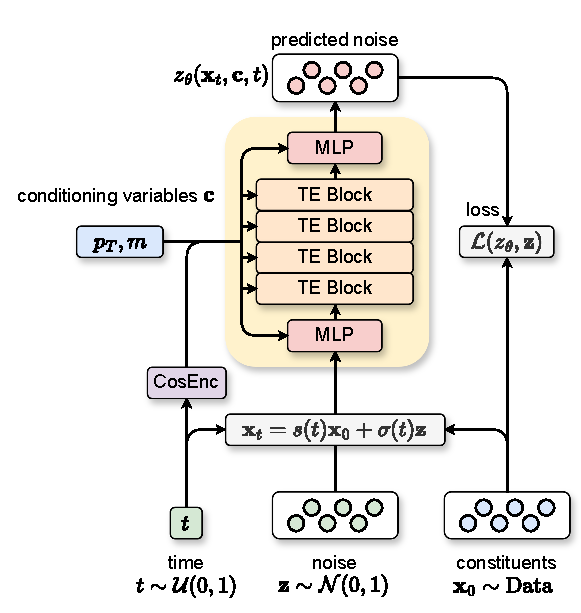
\includegraphics[width=0.65\textwidth]{Figures/jet_generation/pcjedi.pdf}
    \caption{The \pcjedi model architecture configured for training.}
    \label{fig:pcjedi}
\end{figure}

\subsubsection{Integration Solvers}

As with all diffusion models, to generate samples with \pcjedi, numerical integration is required to solve the reverse SDE or the probability flow ODE\@.
This complicates evaluation of the model, as sample quality can vary wildly depending on the solver used, and the number of integration steps taken.
Various numerical solvers for this task~\cite{NumericalSolutionStochastic} are compared.
The Euler-Maruyama (EM) method is used to solve the reverse SDE, and the DDIM sampler~\cite{DDIM} fourth-order Runge-Kutta and Euler methods are used for the probability flow ODE.
Equal step sizes were used for all solvers and negligible differences are observed between ODE solvers.

Generating higher quality samples with a diffusion model requires more integration steps, and thus longer generation times.
For these initial studies the focus was on quality rather than speed, so 200 integration steps were permitted for each jet.

\subsection{Results}

Generated jets are compared to the JetNet30 test set using a variety of metrics
As an additional benchmark for performance, MPGAN~\cite{MPGAN}, a GAN trained on the same dataset, is used.
MPGAN generates the particle cloud with attributes $(\Delta\eta, \Delta\phi, \pt^\text{rel})$, where $\pt^\text{rel} = \pt / \ptjet$.
Therefore, the outputs of \pcjedi are transformed to this format for comparison.
For evaluation, 50,000 jets per class are generated using MPGAN and \pcjedi with the different solvers.

Qualitative performance is assessed by visually inspecting the relative kinematics derived from the generated jets, using $\pt^\text{rel}$ for each constituent.
The overall $\ptpcrel$ and $\mpcrel$ for gluon and top jets are presented in \Cref{fig:kinematics_gluon,fig:kinematics_top}.
Total $\ptpcrel\leq1.0$ due to the trimming of the jet to only the top 30 constituents.
All models struggle to capture the hard cut-off at 1.0, but \pcjedi with DDIM solver shows the closest agreement.
Both \pcjedi methods outperform MPGAN in reconstructing the top jet $\ptpcrel$ distribution, with similar performance in reproducing $\mpcrel$ for all models.

The bi-modal structure observed in top jet $\mpcrel$ arises from a phenomenon in fat jet reconstruction where one of the main parton showers is not contained within the jet radius.
In the case of top jets, stable particles from the $b$-quark decay are sometimes \textit{uncontained}, leading to a jet with a two-pronged structure and masses close to the $W$ boson's mass.

\begin{figure}[hbpt]
    \centering
    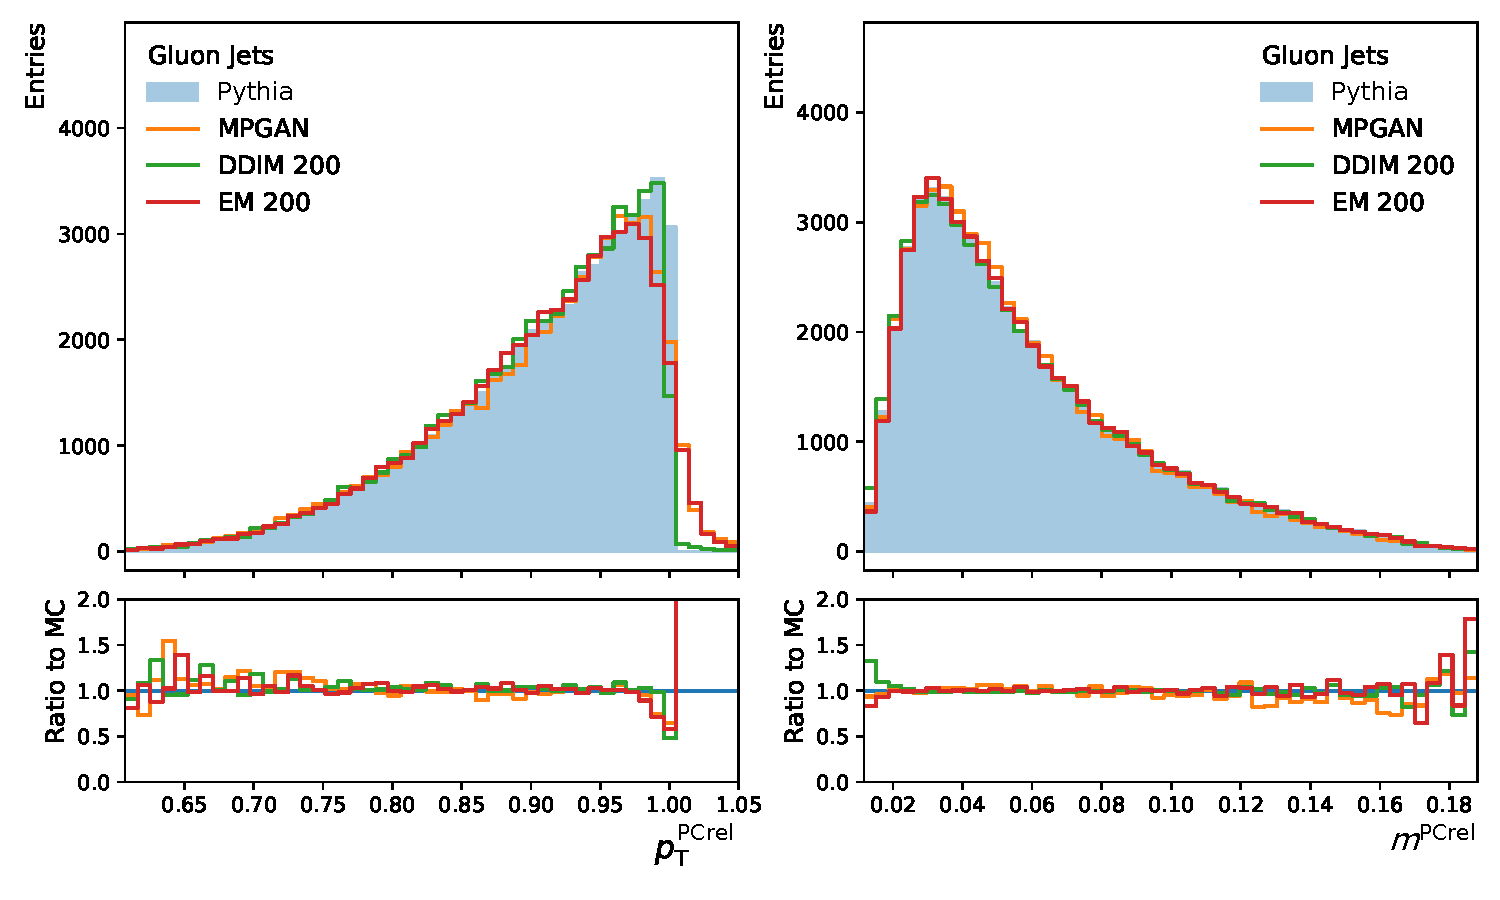
\includegraphics[width=.75\textwidth]{Figures/jet_generation/jedi/gluon/jet_features_rel.pdf}
    \caption{The relative transverse momentum (left) and invariant mass (right) of gluon jets generated with MPGAN and \pcjedi using the DDIM and EM solvers compared to the \pythia simulation. Calculated from the leading 30 \pt constituents using $\pt^\text{rel}$ instead of $\pt$.}
    \label{fig:kinematics_gluon}
\end{figure}

\begin{figure}[hbpt]
    \centering
    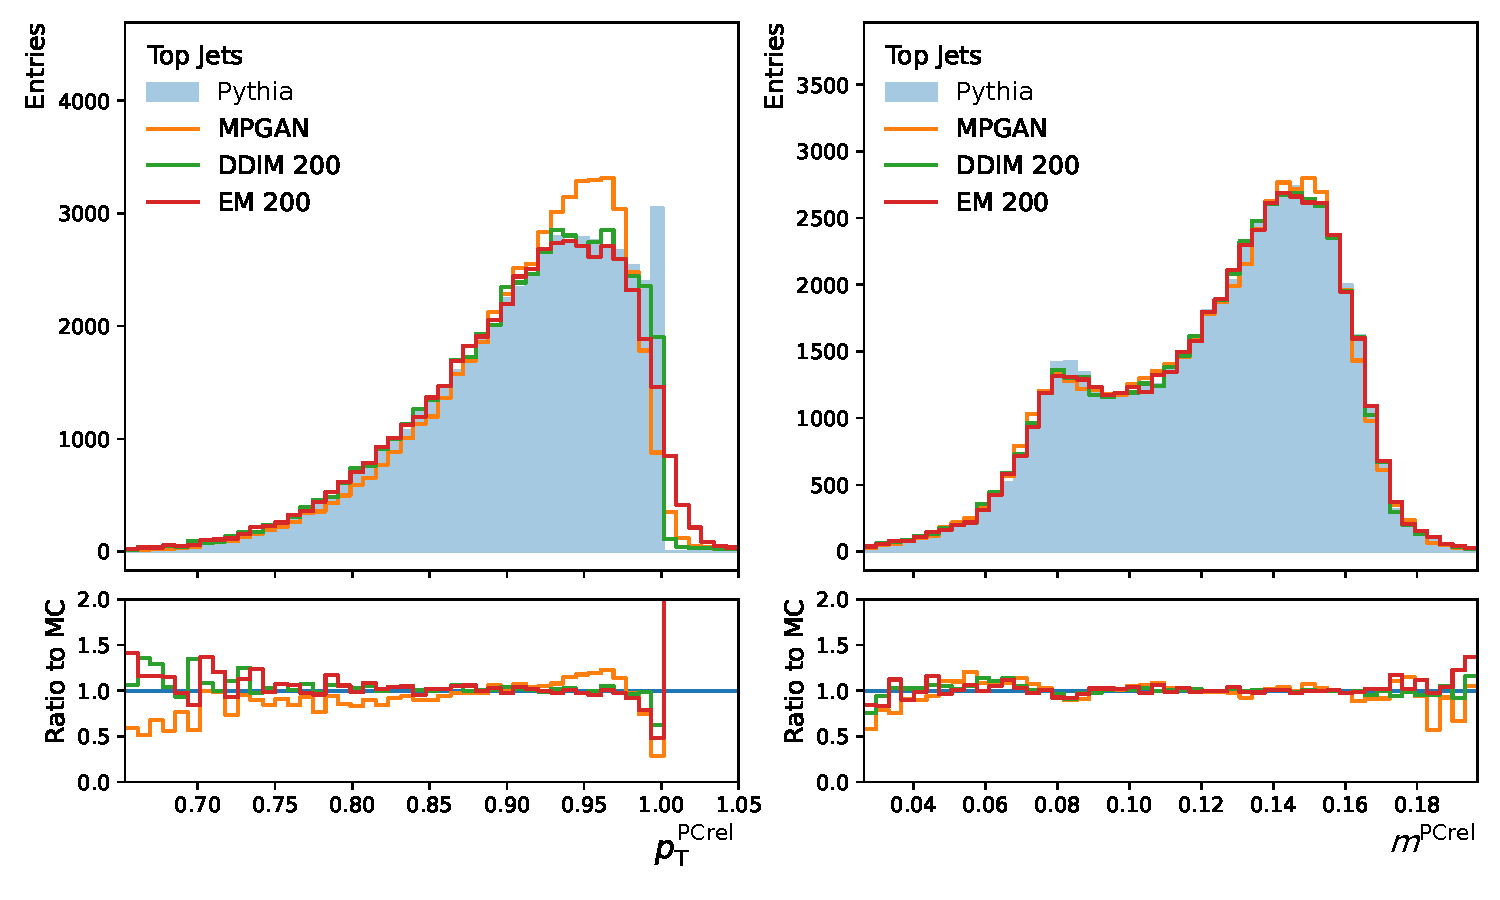
\includegraphics[width=.75\textwidth]{Figures/jet_generation/jedi/top/jet_features_rel.pdf}
    \caption{The relative transverse momentum (left) and invariant mass (right) of top jets generated with MPGAN and \pcjedi using the DDIM and EM solvers compared to the \pythia simulation. Calculated from the leading 30 \pt constituents using $\pt^\text{rel}$ instead of $\pt$.}
    \label{fig:kinematics_top}
\end{figure}

Crucial to the study of large-radius jets are the substructure variables $\tau_{21}$, $\tau_{32}$, and $\Dtwo$, described in \Cref{sec:jet_substructure}\footnote{These variables are already normalized by the jet's total $\pt$, thus relative versions are unnecessary.}.
The subjettiness ratios $\tau_{21}$, $\tau_{32}$ in particular are often used to distinguish the mostly tree-pronged top jets from the one-pronged gluon jets.

Calculated for the generated particle cloud and compared to \pythia simulations, these variables are illustrated in \Cref{fig:substructure_gluon,fig:substructure_top}.
Both \pcjedi and MPGAN models accurately capture the $\text{D}_2$ distributions.
However, all models struggle considerably with $\tau_{21}$ and $\tau_{32}$ especially for top jets, which exhibits a bi-modal structure due to the uncontained $b$-quark decay.

\begin{figure}[hbpt]
    \centering
    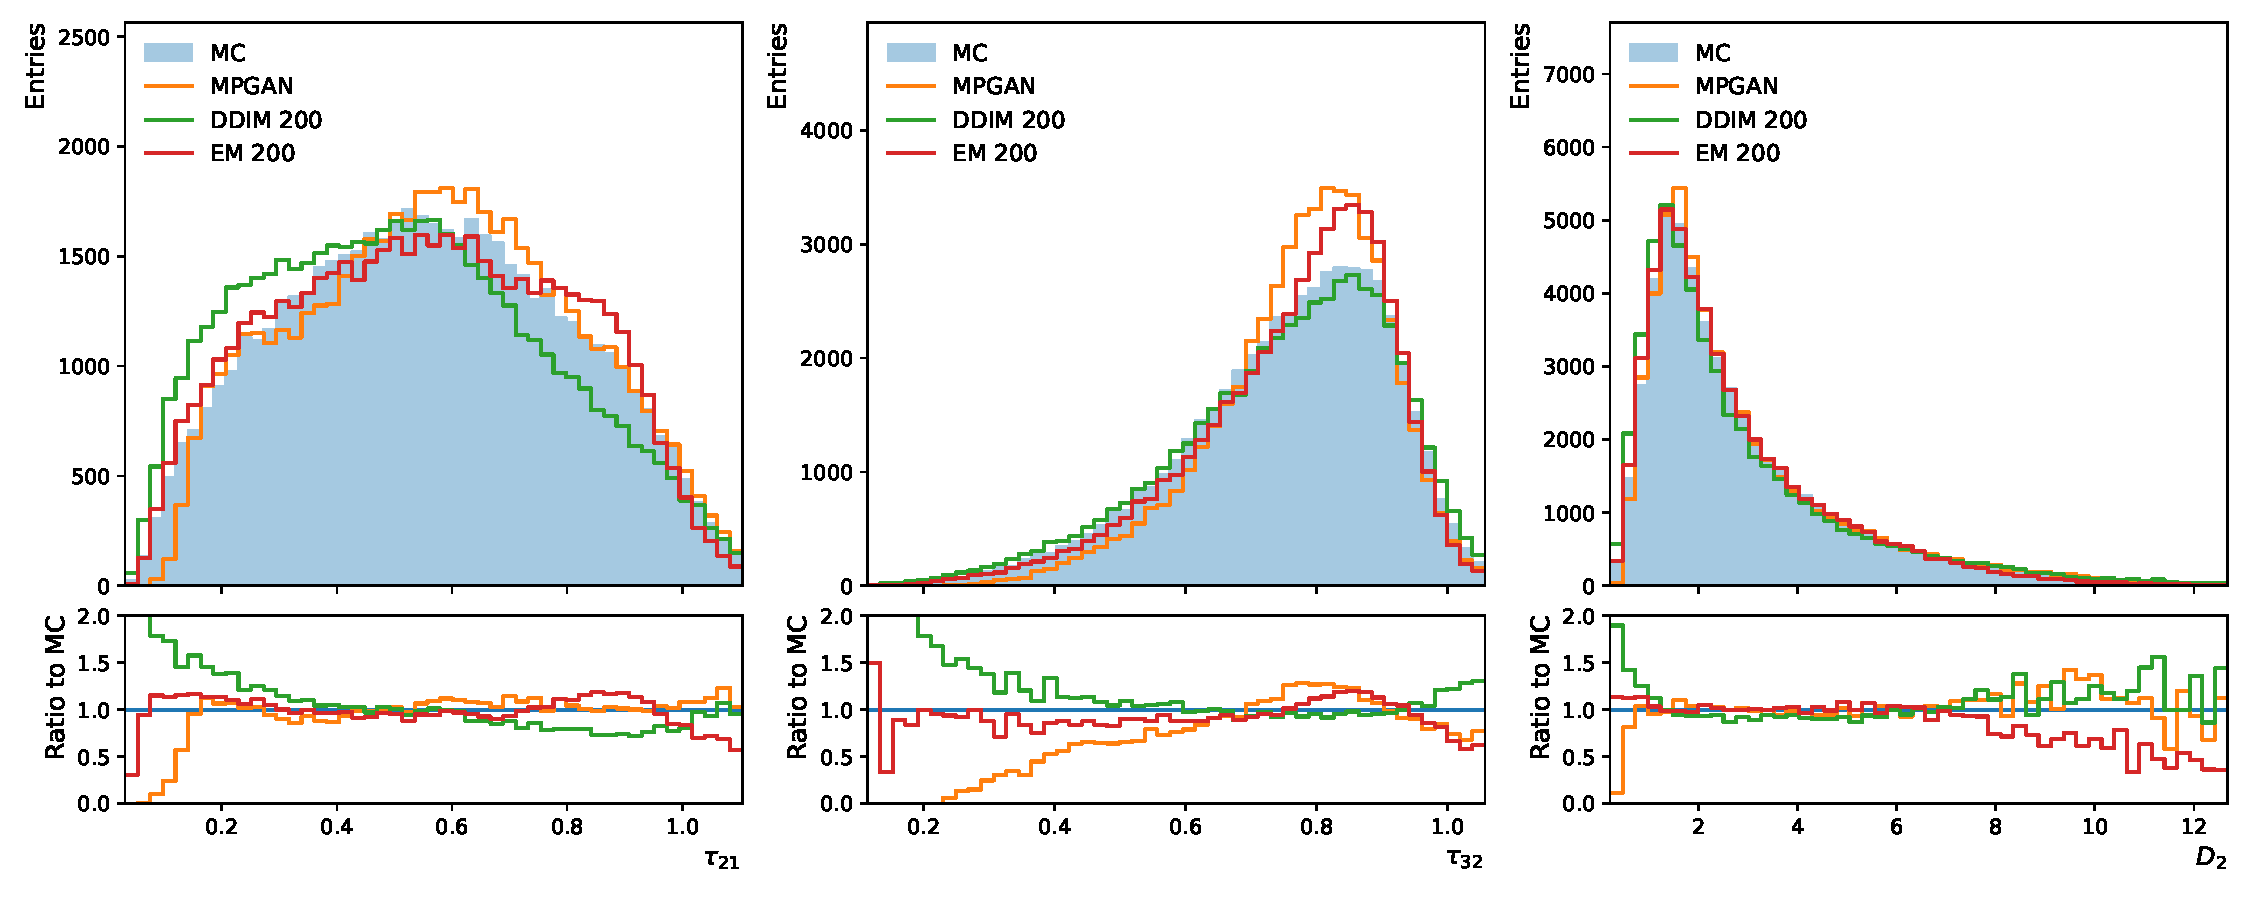
\includegraphics[width=1.\textwidth]{Figures/jet_generation/jedi/gluon/jet_substructure_rel.pdf}
    \caption{Substructure variables of gluon jets generated with MPGAN and \pcjedi using the DDIM and EM solvers compared to the \pythia.}
    \label{fig:substructure_gluon}
\end{figure}

\begin{figure}[hbpt]
    \centering
    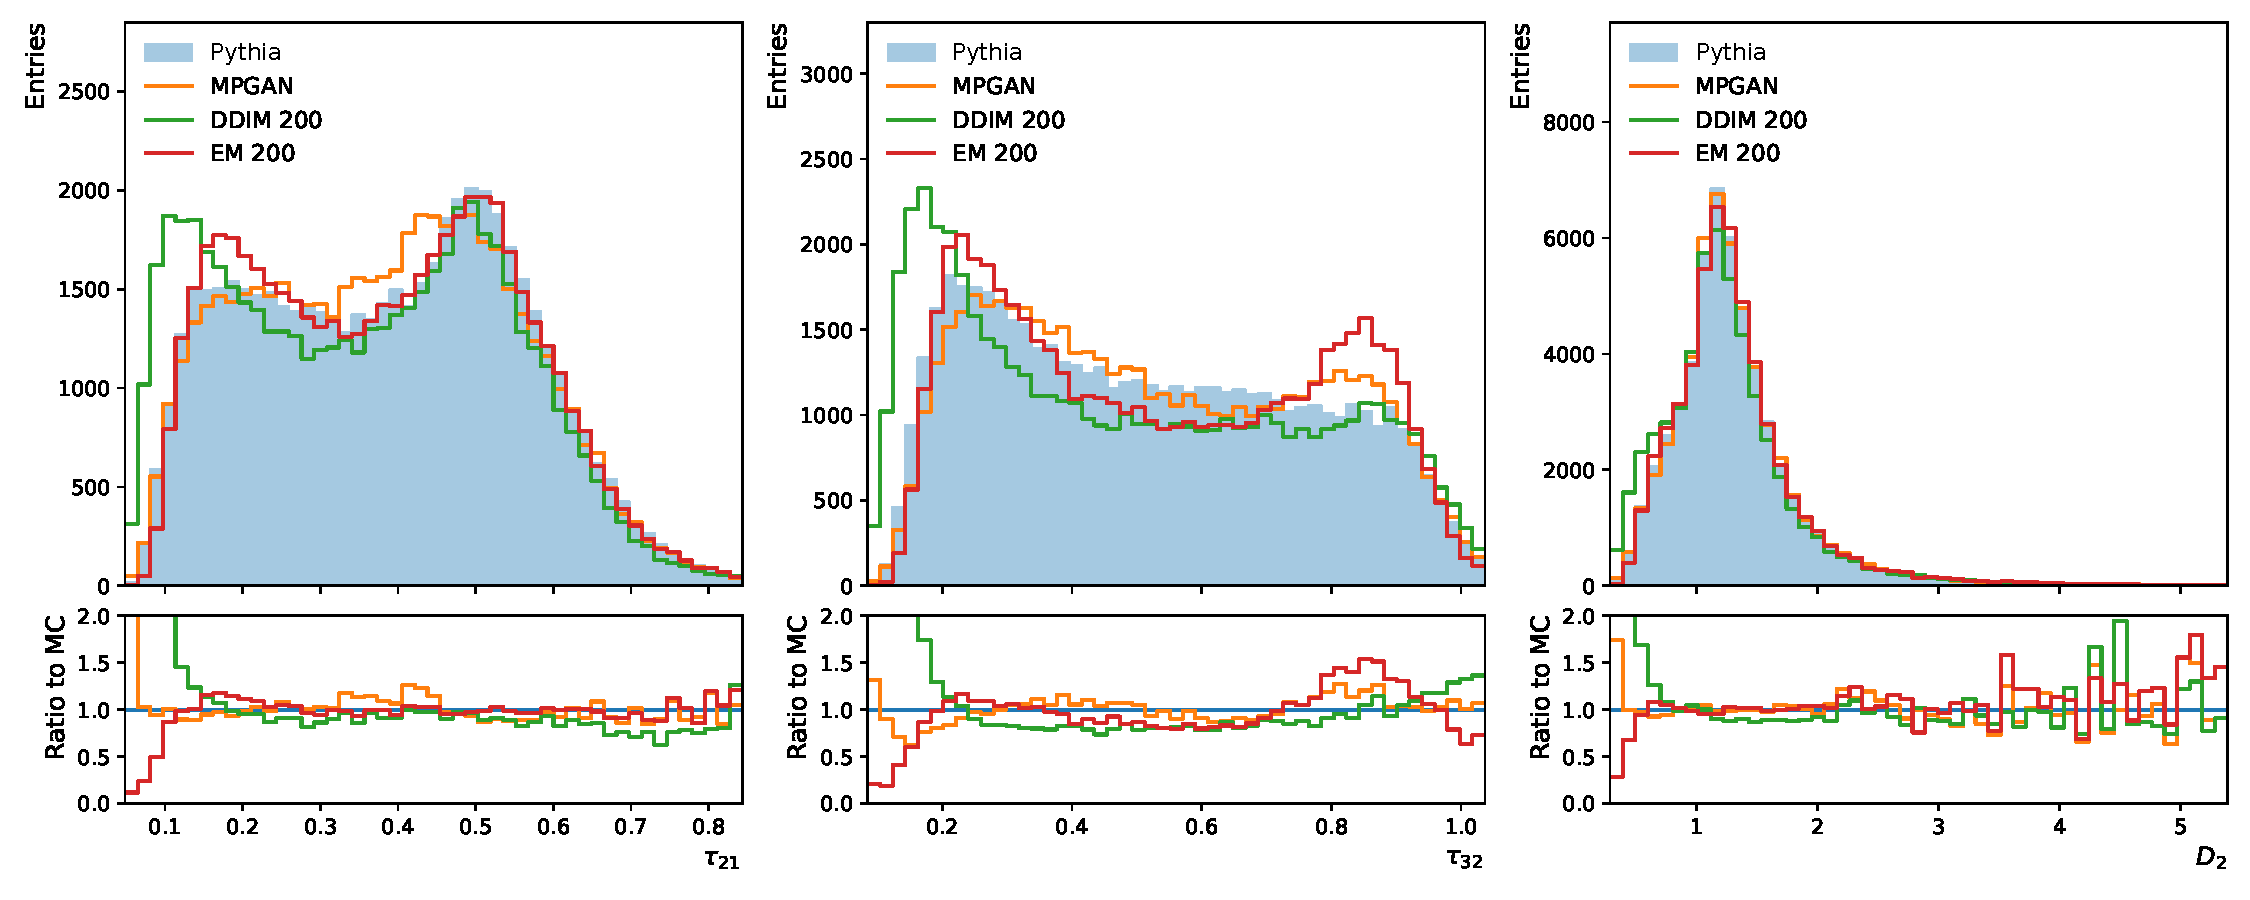
\includegraphics[width=1.\textwidth]{Figures/jet_generation/jedi/top/jet_substructure_rel.pdf}
    \caption{Substructure variables of top jets generated with MPGAN and \pcjedi using the DDIM and EM solvers compared to the \pythia simulation.}
    \label{fig:substructure_top}
\end{figure}

Quantitative metrics are derived following the methodology used in \textcite{MPGAN} whereby the Wasserstein-1 distance is calculated between the generated and \pythia jets.
This creates a $\text{W}_1^X$ score for each observable $X$.
Uncertainties for these scores are derived using bootstrap sampling.
In addition to the distributions shown, a $\text{W}_1$ score is calculated using the average of the first five Energy Flow Polynomials (EFPs)~\cite{EFP}.

The Fréchet ParticleNet distance (FPND) is also calculated for each jet type.
This metric calculates the Fréchet distance between the generated and \pythia jets using the activations of the penultimate layer of the ParticleNet model~\cite{MPGAN, ParticleNet}.

Lower limits for all metrics are calculated by comparing 50k jets from the training set to the test set, which captures the natural variation in the data.
All methods are compared quantitatively in \Cref{tab:combined_results}.
Based on these values, no one model is clearly superior.
\pcjedi with the EM sampler obtains the lower FPND score, but suffers greatly in the EFP distributions for top jets.
MPGAN outperforms \pcjedi in the $\Dtwo$ scores for gluon jets, but not for top jets.
On average, it seems that the EM sampler is worse than the DDIM sampler, at least for the selected 200 integration steps, but the differences are not significant.
One crucial observation is how poorly all models perform on the subjettiness ratios with the values for top jets ranging from around 5 to 10 times higher than the \pythia baseline.
This clearly indicates that the current methods are not sufficient for modelling the substructure of top jets.

\begin{table}[tp]
    \centering
    \caption{Quantitive comparison of the \pcjedi and MPGAN models for generating gluon and top jets.}
    \label{tab:combined_results}
    \renewcommand{\arraystretch}{1.5}
    \resizebox{\textwidth}{!}{%
        \begin{tabular}{llrrrrrr}
    \toprule
    Jet & Model        & FPND            & $\mathrm{W}_1^\mathrm{EFP}$ $(\times 10^{-6})$ & $\mathrm{W}_1^m$ $(\times 10^{-4})$ & $\mathrm{W}_1^{\tau_{21}}$ $(\times 10^{-3})$ & $\mathrm{W}_1^{\tau_{32}}$ $(\times 10^{-3})$ & $\mathrm{W}_1^{\Dtwo}$ $(\times 10^{-2})$ \\
    \midrule
    \multirow{4}{*}{Top}
        & \pythia      & $0.01$          & $8.07 \pm 3.51$                                & $3.23 \pm 1.07$                     & $2.01 \pm 0.74$                               & $2.90 \pm 1.59$                               & $1.16 \pm 0.29$                           \\ \cline{2-8}
        & \pcjedi-EM   & $\mathbf{0.15}$ & $35.61 \pm 4.92$                               & $13.64 \pm 3.21$                    & $4.55 \pm 1.16$                               & $\mathbf{16.05} \pm 1.31$                     & $\mathbf{2.08} \pm 0.40$                  \\
        & \pcjedi-DDIM & $0.28$          & $41.21 \pm 5.61$                               & $14.82 \pm 3.21$                    & $\mathbf{4.40} \pm 1.03$                      & $32.04 \pm 2.29$                              & $2.59 \pm 0.41$                           \\
        & MPGAN        & $0.36$          & $\mathbf{12.80} \pm 4.89$                      & $\mathbf{6.41} \pm 2.09$            & $6.61 \pm 0.92$                               & $17.41 \pm 2.78$                              & $3.40 \pm 0.63$                           \\
    \midrule
    \multirow{4}{*}{Gluon}
        & \pythia      & $0.01$          & $4.07 \pm 1.27$                                & $4.39 \pm 1.59$                     & $3.79 \pm 1.42$                               & $2.26 \pm 0.51$                               & $3.78 \pm 0.70$                           \\ \cline{2-8}
        & \pcjedi-EM   & $\mathbf{0.10}$ & $5.68 \pm 1.09$                                & $\mathbf{5.66} \pm 1.51$            & $12.48 \pm 0.98$                              & $\mathbf{13.32} \pm 0.96$                     & $10.20 \pm 1.04$                          \\
        & \pcjedi-DDIM & $0.12$          & $\mathbf{5.10} \pm 0.99$                       & $9.04 \pm 1.77$                     & $\mathbf{11.99} \pm 1.12$                     & $20.38 \pm 1.91$                              & $11.39 \pm 1.42$                          \\
        & MPGAN        & $0.13$          & $8.76 \pm 2.44$                                & $8.15 \pm 2.10$                     & $16.83 \pm 2.08$                              & $25.27 \pm 1.29$                              & $\mathbf{5.64} \pm 1.01$                  \\
    \bottomrule
\end{tabular}

    }
\end{table}

\subsection{Conclusion}

\pcjedi is the first model to generate particle clouds using a diffusion model, and while the results are promising, they are not state-of-the-art.
Demonstrating the feasibility of this method constitutes a significant step forward.
However, the inability to capture the complex substructure of fat jets remains a notable limitation.
The time required for sample generation is another significant drawback, as diffusion models necessitate multiple forward passes compared to a single pass for GANs.
Additional effort is required to enhance both the performance and speed of the model.

\FloatBarrier

\section{\pcdroid}

This section details the development of \pcdroid~\cite{PCDroid}\footnote{The code repository used in this work is publicly available~\cite{PCDroidCode}}, a successor to \pcjedi.
The \pcdroid model exhibits marked improvements in speed and generation.
Leveraging an updated framework for diffusion models~\cite{ElucidatingDesignSpace}, enhanced diffusion sampling algorithms, and a novel transformer model, \pcdroid better balances performance and generation time.
Additionally, consistency distillation~\cite{ConsistencyModels} is explored to further reduce generation time.
\pcdroid achieves state-of-the-art performance on the benchmarks discussed in the previous section, significantly surpassing both \pcjedi and MPGAN.
More comprehensive timing studies are presented with compare the various models against \pythia.

\subsection{Improved Diffusion Framework}

One of the main advancements in \pcdroid is the revised diffusion paradigm and configuration.
\pcdroid adheres to the EDM noise scheduler and network preconditioning as outlined by \textcite{ElucidatingDesignSpace} and discussed in \Cref{sec:diffusion_frameworks}.
This approach introduces several key modifications.

Firstly, the signal and noise rates are defined as $\gamma(t)=1$ and $\sigma(t)=t$.
This adjustment simplifies the forward SDE to
\begin{equation}
    \diff \x_t = \sqrt{2t} \diff \w_t,
\end{equation}
with the corresponding ordinary differential equation ODE similarly reducing to,
\begin{equation}
    \diff x_t = - t \score \diff t.
\end{equation}
As a result, the ODE solutions exhibit straighter trajectories, reducing truncation errors during generation compared to the previous variance-preserving method.
The primary advantage of this change is the ability to execute the reverse diffusion process in fewer steps.

Secondly, diffusion times are sampled during training specifically to target regions of the diffusion process where the model can gain the most information.
These diffusion times are used to scale the noise added to the input data.
Note that the diffusion time $t$ and noise rate $\sigma(t)$ can be used interchangeably.
They are now defined in the range $t = \sigma(t) \in [0, 80]$.
When $t$ is low, the magnitude of the artificial noise introduced into the samples is indistinguishable from the inherent stochasticity of the data.
Conversely, at high values of $t$, the input sample is almost entirely corrupted by noise, and the model can not be expected to recover any meaningful information.
Log-normal sampling of the diffusion times, ${\log(t)\sim\mathcal{N}\left(-1.2, 1.2\right)}$, preferentially targets intermediate values where the model can learn the most.

Thirdly, skip and scaling connections are integrated into the network architecture.
The variables $c_\mathrm{in}(t)$, $c_\mathrm{out}(t)$, and $c_\mathrm{skip}(t)$ are all parameterized by $t$ and are combined for the denoised estimate as follows:
\begin{equation}
    x_\theta(\x, \cond, t) = c_\mathrm{out} f_\theta(c_\mathrm{in}\x, \cond, t) + c_\mathrm{skip}\x,
\end{equation}
where $f_\theta$ represents the raw prediction from the neural network.
Note that unlike \pcjedi, the target for the network is the true data sample $\x_0$ rather than the noise $\z$.
The skip connection permits $\x_t$ to bypass the network at low $t$, as the input is already close to the target.
Due to the variance not being preserved during the diffusion process, these scaling functions maintain the unit variance of the raw inputs and targets
for $f_\theta$.

The same dataset, JetNet30, as outlined in \Cref{sec:jetgen_data}, is reused for some experiments in this section.
However, most studies utilize the extended JetNet150 dataset, which encompasses the same jets, but with up to 150 constituents within the particle cloud.
This expanded dataset introduces new challenges for the generative task, necessitating more intricate models and increased computational resources to manage the larger set size effectively.
Additionally, all five jet types in JetNet150 are used ($q,\,g,\,t,\,W,\,Z$).

\subsection{Model Architecture}

The general \pcdroid architecture and the training process is shown in \cref{fig:droid_arch_train}.

\pcdroid incorporates an additional MLP compared to \pcjedi.
The context vector is expanded to include the jet azimuthal angle ($\phi$), the number of constituents (which was previously only implicitly included in the input set size), and the jet type (PID).
The new MLP processes this vector before sending it to each sublayer.
Conditioning on the jet type is significant because, unlike \pcjedi and MPGAN, which required separate models for each jet type, \pcdroid can generate all five jet types with a single network.
Moreover, the conditioning features represent the full jet kinematics rather than just the net kinematics of the particle cloud.
Consequently, the generation task becomes more challenging, as the model must learn the effects of trimming the constituents.

\begin{figure}[htpb]
    \centering
    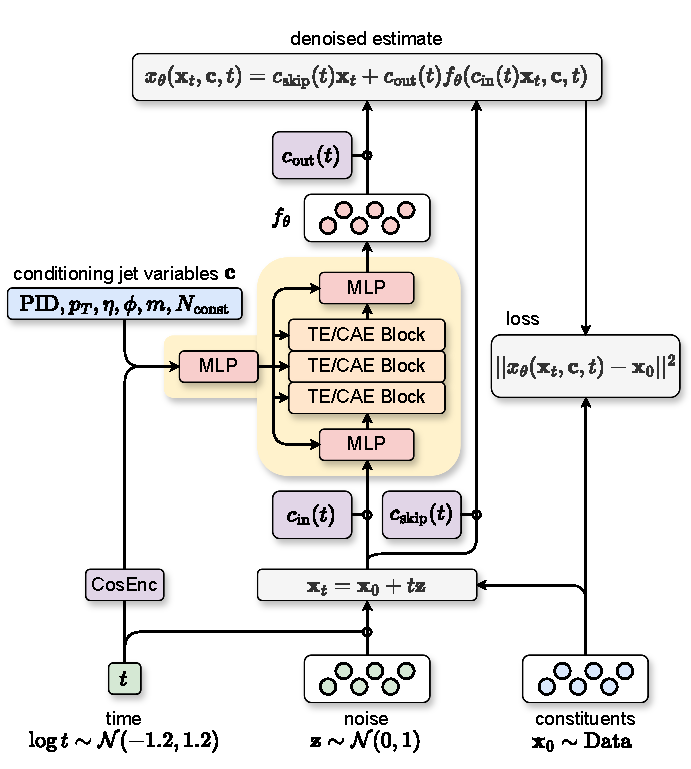
\includegraphics[width=0.6\textwidth]{Figures/jet_generation/pcdroid.pdf}
    \caption{The \pcdroid model architecture configured for training.}
    \label{fig:droid_arch_train}
\end{figure}

In \pcjedi, only TE Blocks with self-attention are studied, which, despite their high expressiveness, are computationally expensive.
The number of operations scales quadratically with the number of constituents $N_{const}$, i.e., $\mathcal{O}(N_{const}^2)$.
Given that diffusion models necessitate multiple network passes during generation, self-attention becomes a suboptimal choice for fast generation.
This computational demand is highly significant when scaling to 150 constituents.
Consequently, alongside the TE based model, the cross-attention encoder (CAE) is introduced, which serves as a more efficient and memory-conserving permutation-equivariant network.

A schematic overview of the CAE Block is illustrated in \Cref{fig:cae_network}.
In this network layer, the input set updates a collection of global tokens via multi-headed cross-attention.
These tokens are then refined through a residual MLP and redistributed back to the input set using another cross-attention layer and residual MLP.
The layer therefore has two cross-attention operations, one to ``pool'' information from the input set into the global tokens and another to ``distribute'' information back to the input set.
The CAE's attention operations scale with $\mathcal{O}(N_{const} \times N_{global})$.
The full CAE is constructed by sequentially stacking multiple CAE Blocks, with the initial set of global tokens being fully learnable.
The number of global tokens $N_{global}$ is as a hyperparameter and for $N_{global}=1$, the distribute attention operation employs a sigmoid function instead of softmax.

\begin{figure}[htpb]
    \centering
    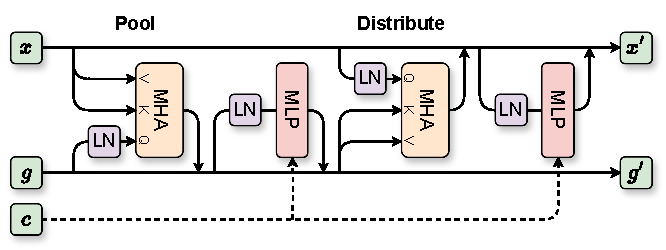
\includegraphics[width=0.8\textwidth]{Figures/jet_generation/CAEB.pdf}
    \caption{A single cross-attention encoder block updating both an input point cloud $x$ and global tokens $g$, using layer-norm (LN), multi-headed attention (MHA). Contextual information $c$ is injected into the network by concatenating to the inputs of the MLPs.}
    \label{fig:cae_network}
\end{figure}

To allow direct comparisons with \pcjedi, the optimizer, learning rate, scheduler, and the majority of hyperparameters remain unchanged.
The only notable adjustments, based on a minor hyperparameter scan, include reducing the number of encoder layers from four to three and using MSE loss for training.
For models with 150 constituents, the token dimension and the width of the MLP layers were doubled.
Two additional models utilizing CAE Blocks with $N_{global}=1$ and $N_{global}=16$ are trained on the 150 constituent dataset, employing the same training configuration, dimensions, and number of layers as the baseline model.

\subsubsection{Integration Solvers}

Another key development in \pcdroid has been in the choice of integration solvers used during inference.
As the mechanisms for sampling from the diffusion process are an area of active research, it is challenging to keep up with and support all the latest advancements. Therefore, \pcdroid was designed to be compatible with the popular \textsc{KDiffusion} library~\cite{KDiffusion} and thus can utilize any of the samplers made available there.
These samplers operate on either the reverse SDE or the probability flow ODE.

The most promising methods include the Heun's method on both the ODE and SDE~\cite{ODEBook}, DPM-Solver-2~\cite{DPMSolverFastODE}, DPM-Solver++~\cite{DPMSolverFastSolver}, and DPM-Solver-2M~\cite{DPMSolverFastSolver}, a fourth order linear multistep method (LMS)~\cite{ODEBook} and ancestral sampling variants of these.
Furthermore, experimenting with non-uniform step sizes during generation reveals that systematically taking larger steps at the beginning of the denoising process and smaller steps towards the end improves the quality of the generated samples.

\subsection{Consistency Distillation}

This work investigated the process of consistency distillation (CD)~\cite{ConsistencyModels}, wherein a teacher network trains a student network to solve the reverse diffusion process in fewer steps, and in some cases enabling one-step generation.

The teacher network is a standard pre-trained diffusion model.
Combined with a sampling method, it traces paths along the learned probability flow ODE.
During distillation, the weights of the teacher network are frozen.
A student network is then trained to map all points sampled along the same ODE trajectory to a constant output.
This target is not required to be the end point of the trajectory, as this would require fully solving the ODE for each training step.
To prevent the student model from collapsing, a boundary condition is enforced whereby the student must become an identity map as $t \rightarrow 0$.
The $c_\text{skip}$ and $c_\text{out}$ preconditions used in the EDM framework already enforce this.
This boundary condition ensures the global minimum of the training loss is achieved only when the student network maps each point of the ODE trajectory to its endpoint.

The student model is initialized with the same parameter values as the teacher.
During training, the diffusion time is sampled, the input is corrupted using the same schedule as before, and then the teacher model is used to take a single step along the ODE.
These two adjacent points on the ODE are each passed through the student network, and the student is trained to minimize the mean squared distance between its two outputs.
To stabilize training, the student network is duplicated into an online and target network, a practice common in deep reinforcement learning~\cite{PlayingAtariDeep, ContinuousControlDeep, ImplicitQuantileNetworks}.
Gradients are propagated only through the online network, which always processes the ODE sample with the larger $t$.
After each iteration, the target network is synced with the online network using an exponential moving average of the parameters.

CD is similar to progressive distillation (PD)~\cite{ProgressiveDistillationFast}, but with key differences.
In PD, new models are iteratively trained to predict the noise removed in $N$ steps of the previous model.
This process reduces the number of steps required with each new model, leading to faster generation times.
Unlike CD, PD does not need information about the ODE trajectories, only the total noise removed after $N$ steps.

\subsection{Unconditional Generation}

\pcdroid is a conditional generative model, where the conditions include the jet kinematics $(\pt, \eta, \phi, m)$, the number of constituents ($N_{const}$), and the jet type PID.
For unconditional generation, a second generative model is produced for these variables.
As this is a low-dimensional vector, a normalizing flow (NF) is ideal for this task.
This approach is preferable to explicitly unconditional models as it logically segments the learning process.

Standard use cases would still demand control over the jet type, so
one flow (Flow-$\p$) is trained to learn the probability density $p(\pt, \eta, m, N_{const} |\textrm{PID})$.
As the main model denoises all input tokens, the number of constituents is always required at generation time.
A second flow (Flow-$N$) is trained to learn the probability density $p(N_{const}|\pt, \eta, m, \textrm{PID})$.
As $N_{const}$ correlates with many jet properties, a NF is necessary rather than sampling from a Poisson distribution.
This second flow demonstrates how \pcdroid can be used as a surrogate fast simulator, especially when the parton type and kinematics are known, but the number of particles in the final jet is not.

Both flows are trained with a maximum log-likelihood objective and consist of five transformation layers using rational quadratic splines~\cite{NeuralSplineFlows}.
Coupling layers are used in Flow-$\p$, while none are needed for the one-dimensional transformation in Flow-$N$.
For both flows, a dequantization step simplifies the learning of the $N_{const}$ distribution; at inference time, the generated value is rounded to the nearest integer.
The Adam optimizer~\cite{Adam} with default settings and a cosine learning rate is used.
Given the relatively simple nature of these distributions, near-perfect performance is achieved.

\subsection{Results on JetNet30}

The \pcdroid, \pcjedi, and MPGAN models are compared on the JetNet30 dataset using the same distributions and metrics as before.
This study uses \pcdroid samples generated under the fully conditional regime.

A wide variety of integration solvers are tested for \pcdroid.
The trade-off between the quality of generated jets and the number of neural function evaluations (NFE) is studied to determine the optimal solver and step size.
The comparison focuses on the FPND, $\mathrm{W}_1^m$, and $\mathrm{W}1^{\tau{32}}$ metrics.
For \pcjedi, the results using the Euler-Maruyama sampler at 200 NFE are used.
From \cref{fig:metrics_vs_steps-30}, most solvers are observed to saturate around 100 NFE.
\pcdroid outperforms MPGAN with as few as 20 steps for most solvers.
Although no method is clearly superior, the LMS solver generally performs best across most metrics and is thus used at 100 NFE for all \pcdroid results in the following sections.

\begin{figure}[tb]
    \centering
    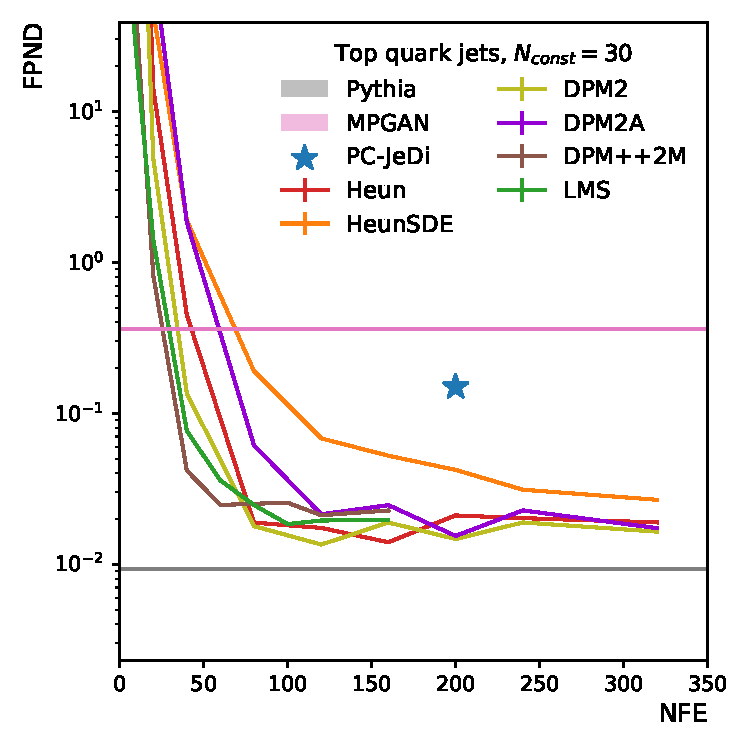
\includegraphics[width=0.32\textwidth]{Figures/jet_generation/droid/30/metrics_vs_steps/t/t_fpnd.pdf}
    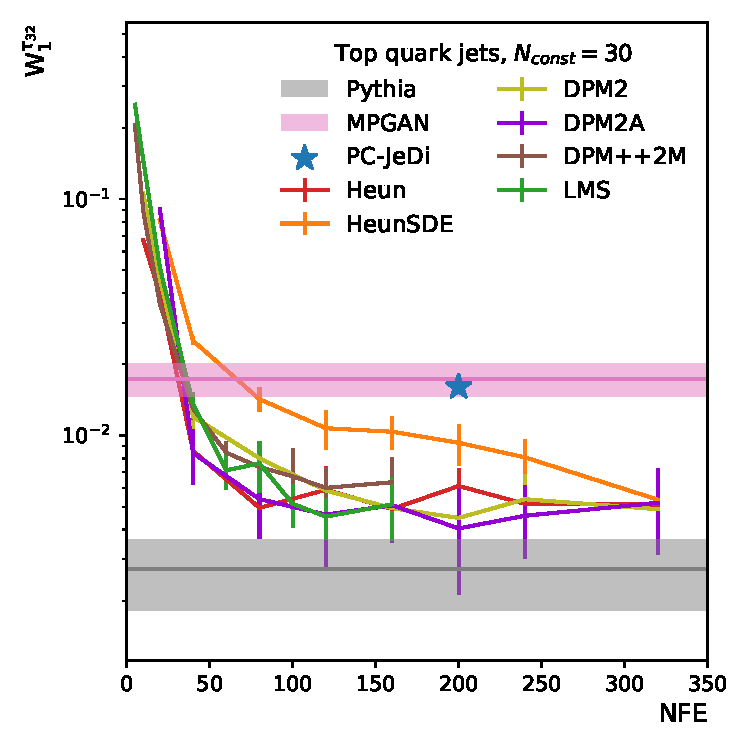
\includegraphics[width=0.32\textwidth]{Figures/jet_generation/droid/30/metrics_vs_steps/t/t_w1_tau_32.pdf}
    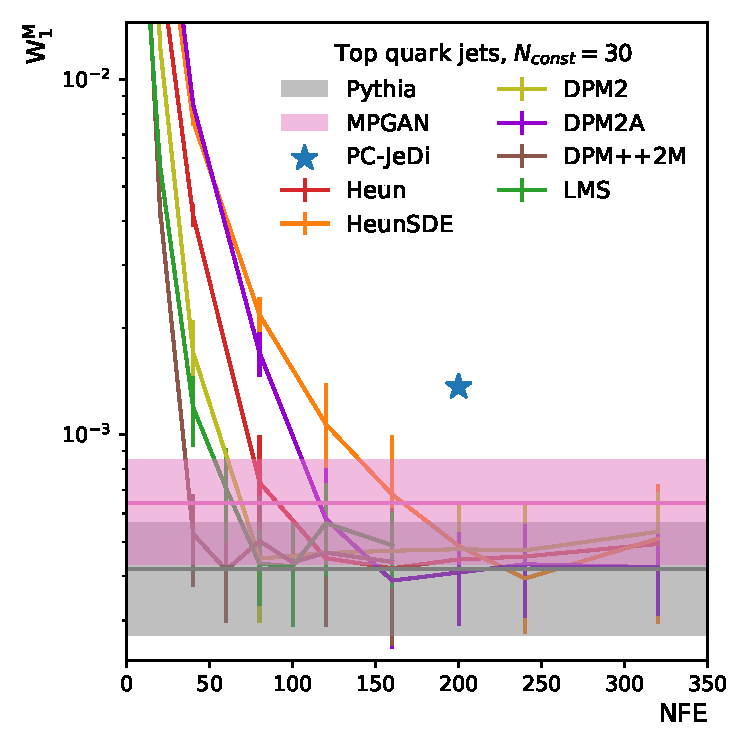
\includegraphics[width=0.32\textwidth]{Figures/jet_generation/droid/30/metrics_vs_steps/t/t_w1m.pdf}
    \caption{Performance as measured by FPND (left), W$_1^{\tau_{32}}$ (middle), and W$_1^m$ (right) as a function of the NFE used during generation for the \pcdroid model for top jets with up to 30 constituents.}
    \label{fig:metrics_vs_steps-30}
\end{figure}

Effectively modelling the kinematics of individual constituents is essential for jet generation.
\Cref{fig:const-pt_dist-30} illustrates the \pt distributions of the leading, fifth leading, and twentieth leading constituents of the generated top and gluon jets, as represented by \pcdroid and \pcjedi.
\pcdroid shows better alignment with \pythia compared to \pcjedi across all constituents, especially in the distribution tails.

\begin{figure}[htpb]
    \centering
    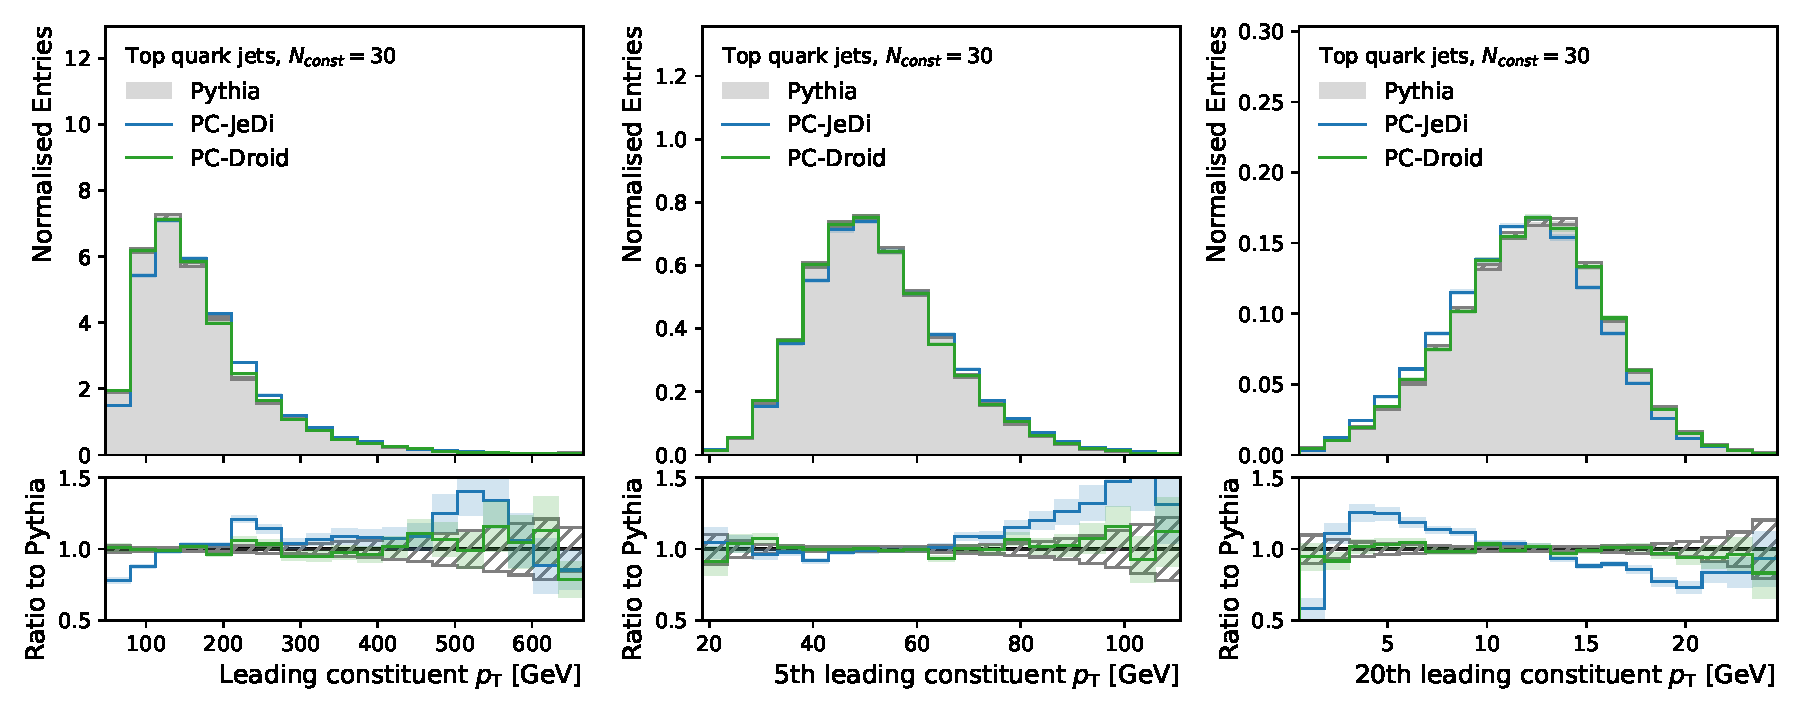
\includegraphics[width=0.99\textwidth]{Figures/jet_generation/droid/30/csts/t/100/t_leading_constituents.pdf} \\
    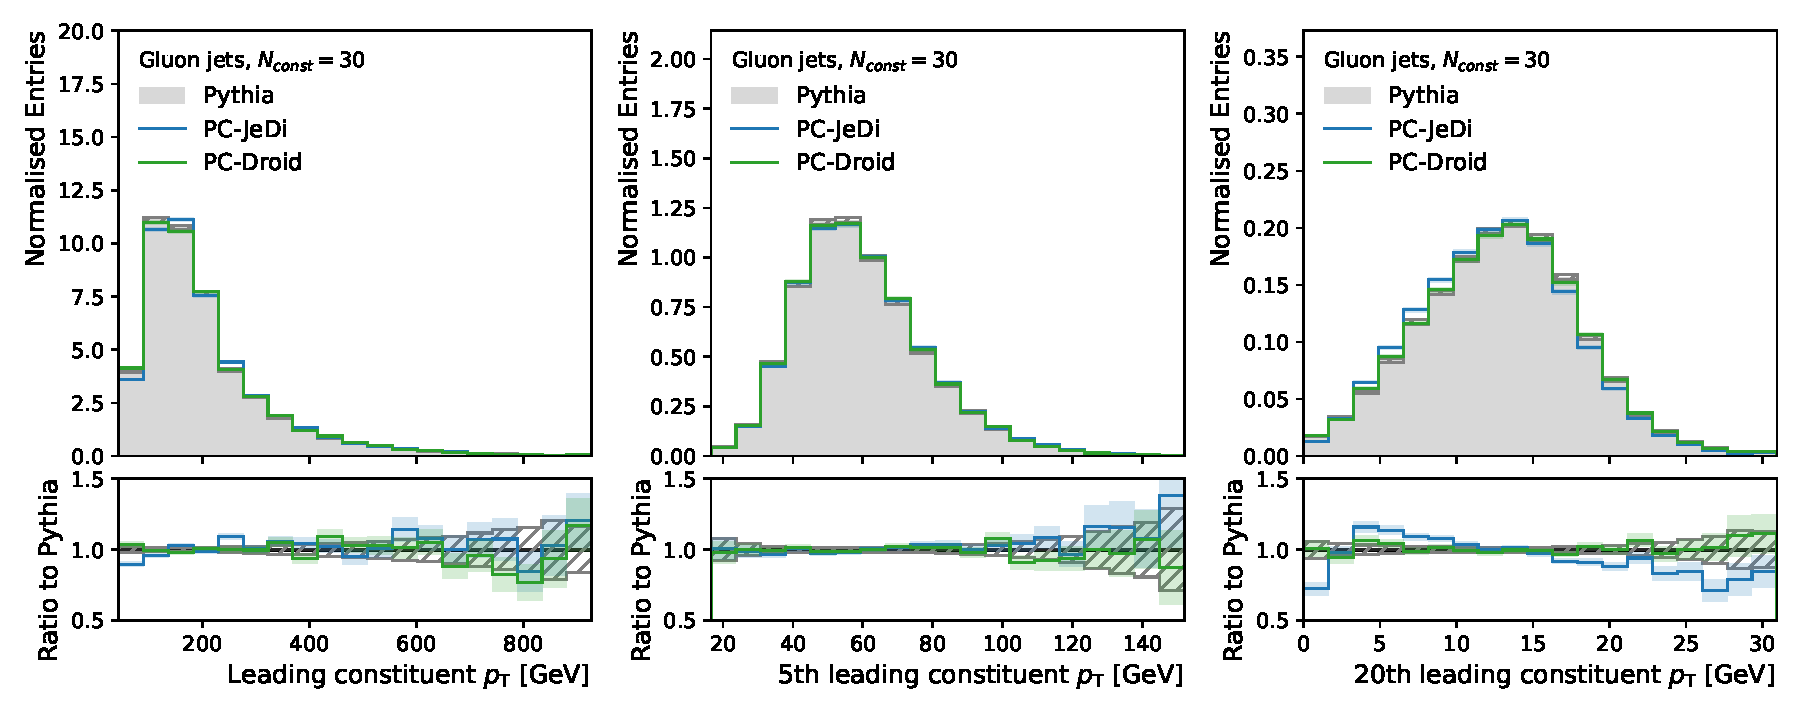
\includegraphics[width=0.99\textwidth]{Figures/jet_generation/droid/30/csts/g/100/g_leading_constituents.pdf}
    \caption{Comparison of \pt distributions of the leading, fifth leading, and twentieth leading constituents of the generated top and gluon jets with up to 30 constituents.}
    \label{fig:const-pt_dist-30}
\end{figure}

Next, the substructure variable distributions of the generated jets and their correlations, essential for jet tagging, are examined.
Focus is on top jets due to their complex substructure, which has proven challenging to model.
\Cref{fig:hlvs-30} shows that \pcdroid significantly improves $\tau_{32}$ modelling compared to \pcjedi and aligns excellently with \pythia simulations for all other substructure variables.

\begin{figure}[htpb]
    \centering
    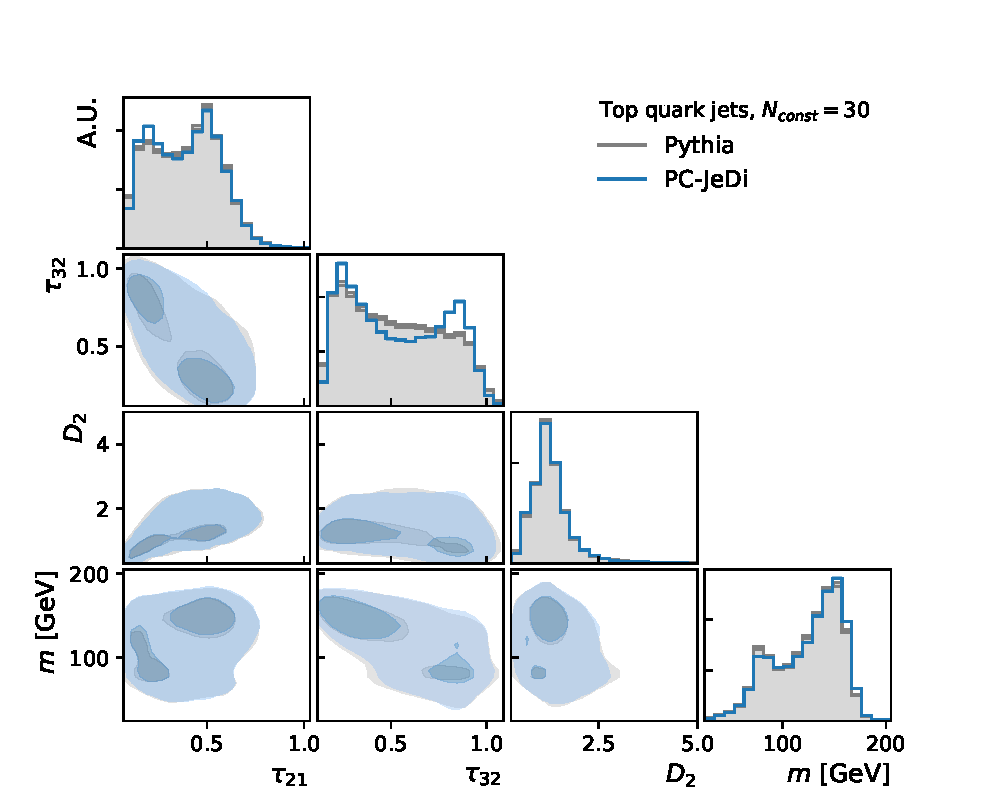
\includegraphics[width=0.49\textwidth]{Figures/jet_generation/droid/30/hlvs/t/100/hlv_corr_PC-Jedi.pdf}
    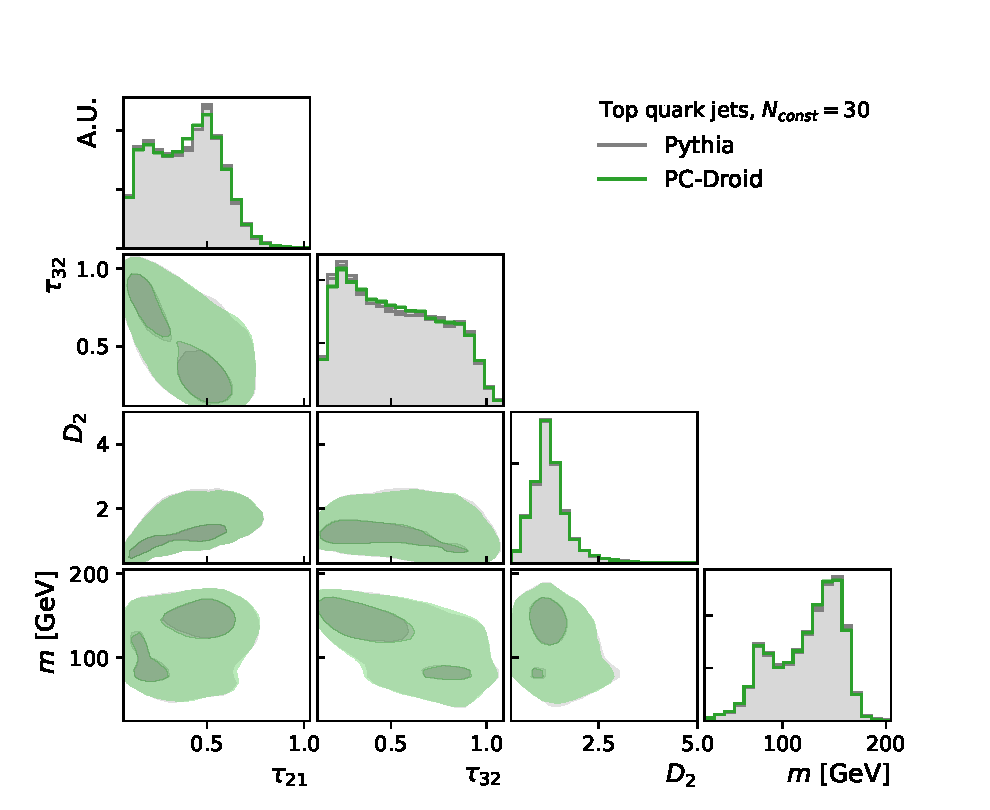
\includegraphics[width=0.49\textwidth]{Figures/jet_generation/droid/30/hlvs/t/100/hlv_corr_PC-Droid.pdf}
    \caption{
        Mass and substructure distributions of the generated top jets with up to 30 constituents.
        The diagonal consists of the marginals of the distributions and the off-diagonal elements contain the joint distributions.
    }
    \label{fig:hlvs-30}
\end{figure}

The generation performance is summarized in~\cref{tab:30_table} for gluon and top jets.
The $\mathrm{W_1^P}$ score is derived from the marginal distributions of the constituent kinematics.
Particularly in FPND, \pcdroid surpasses all other methods in all metrics, reaching the intra MC-MC comparison limits in the subjettiness ratios for gluons and $\mathrm{W_1^{\Dtwo}}$ for both jet types.

\begin{table}[tp]
    \centering
    \caption{Comparison of generative models on top and gluons with up to 30 constituents. Lower is better.}
    \label{tab:30_table}
    \renewcommand{\arraystretch}{1.5}
    \resizebox{\textwidth}{!}{%
        \begin{tabular}{llrrrrrrr}
    \toprule
    Jet & Model    & FPND            & $\mathrm{W_1^P}$ $(\times 10^{-4})$ & $\mathrm{W}_1^\mathrm{EFP}$ $(\times 10^{-6})$ & $\mathrm{W}_1^m$ $(\times 10^{-4})$ & $\mathrm{W}_1^{\tau_{21}}$ $(\times 10^{-3})$ & $\mathrm{W}_1^{\tau_{32}}$ $(\times 10^{-3})$ & $\mathrm{W}_1^{\Dtwo}$ $(\times 10^{-2})$ \\
    \midrule
    \multirow{4}{*}{Top}
        & \pythia  & $0.01$          & $3.98 \pm 1.27$                     & $8.07 \pm 3.51$                                & $3.23 \pm 1.07$                     & $2.01 \pm 0.74$                               & $2.90 \pm 1.59$                               & $1.16 \pm 0.29$                           \\ \cline{2-9}
        & \pcdroid & $\mathbf{0.02}$ & $\mathbf{5.02 \pm 1.59}$            & $\mathbf{11.59 \pm 3.29}$                      & $\mathbf{4.27 \pm 1.39}$            & $\mathbf{2.91 \pm 1.09}$                      & $\mathbf{5.14 \pm 1.06}$                      & $\mathbf{1.26 \pm 0.33}$                  \\
        & PC-JeDi  & $0.15$          & $12.07 \pm 2.01$                    & $35.61 \pm 4.92$                               & $13.64 \pm 3.21$                    & $4.55 \pm 1.16$                               & $16.05 \pm 1.31$                              & $2.08 \pm 0.40$                           \\
        & MPGAN    & $0.36$          & $21.73 \pm 2.02$                    & $12.80 \pm 4.89$                               & $6.41 \pm 2.09$                     & $6.61 \pm 0.92$                               & $17.41 \pm 2.78$                              & $3.40 \pm 0.63$                           \\
    \midrule
    \multirow{4}{*}{Gluon}
        & \pythia  & $0.01$          & $3.54 \pm 1.19$                     & $4.07 \pm 1.27$                                & $4.39 \pm 1.59$                     & $3.79 \pm 1.42$                               & $2.26 \pm 0.51$                               & $3.78 \pm 0.70$                           \\ \cline{2-9}
        & \pcdroid & $\mathbf{0.01}$ & $\mathbf{3.66 \pm 1.07}$            & $\mathbf{4.13 \pm 1.61}$                       & $\mathbf{4.48 \pm 1.47}$            & $\mathbf{2.89 \pm 0.80}$                      & $\mathbf{1.99 \pm 0.51}$                      & $\mathbf{3.52 \pm 1.33}$                  \\
        & PC-JeDi  & $0.10$          & $5.83 \pm 1.44$                     & $5.68 \pm 1.09$                                & $5.66 \pm 1.51$                     & $12.48 \pm 0.98$                              & $13.32 \pm 0.96$                              & $10.20 \pm 1.04$                          \\
        & MPGAN    & $0.13$          & $10.26 \pm 1.51$                    & $8.76 \pm 2.44$                                & $8.15 \pm 2.10$                     & $16.83 \pm 2.08$                              & $25.27 \pm 1.29$                              & $5.64 \pm 1.01$                           \\
    \bottomrule
\end{tabular}

    }
\end{table}

\FloatBarrier

\subsection{Results on JetNet150}

The JetNet150 dataset poses a more challenging task, both due to the increased number of constituents and the inclusion of all five jet types.
For plots, the focus is on top jets as they are the most challenging to model, but metrics are derived for all types.

The marginals of the leading, fifth leading, and twentieth leading constituents of the generated jets are shown in \Cref{fig:const-pt_dist-150}.
Both the original transformer-based model and CAE networks with 1 and 16 global tokens, labeled CAE-1 and CAE-16, are evaluated.
The LMS sampling method at 100 NFE yields similarly optimal results for both networks and is used to derive all subsequent results.
Almost all methods performed sufficiently well in this task.
Substructure distributions are displayed in Figure \Cref{fig:hlvs-150-marginals}.
A comparison of high-level correlations between the transformer and CAE-1 models is shown in \Cref{fig:hlvs-150}.
Both models accurately capture jet mass and $\Dtwo$, though CAE-1 exhibits slightly diminished performance in subjettiness ratios.

MPGAN was never developed for 150 constituents.
As benchmarks for this dataset, comparisons are made to two other deep generative models: FPCD~\cite{FPCD} and EPiC-GAN~\cite{EPICGAN}.

FPCD is a diffusion model developed concurrently with \pcdroid.
It trains on all jet types simultaneously and can produce jets with up to 150 constituents.
FPCD uses different network layers, diffusion schedule, and framework compared to \pcdroid. It jointly trains a single model to produce both high-level kinematics and low-level constituents.
This procedure is fairly inefficient, as for unconditional generation FPCD it must first sample from the former, which is then used as a condition for sampling the latter.
Both steps require numerical integration.
Furthermore, sampling the high-level features is an orthogonal task and does not need to share the same network layers or noise seed as the rest of the model.
FPCD was progressively distilled to perform generation in a single step.

EPiC-GAN is a GAN model using specially designed layers.
Instead of conventional message passing, EPiC layers pool information from all nodes to a global vector and then concatenate this to all nodes during the updates in the following layer.
It is essentially a repeated implementation of a deep set and shares similarities with the CAE-1 model.
In EPiC-GAN, a kernel-density estimator (KDE) models the number of constituents, which is a conditional parameter for generation.

A quantitative comparison of the performance of \pcdroid and all other models is provided in \cref{tab:perf-150}.
\pcdroid with the self-attention network shows superior performance in all metrics across all jet types wherever there is notable separation between models.
Where performance is saturated, the CAE-1 or CAE-16 models are comparable to the transformer model.

\begin{figure}[tb]
    \centering
    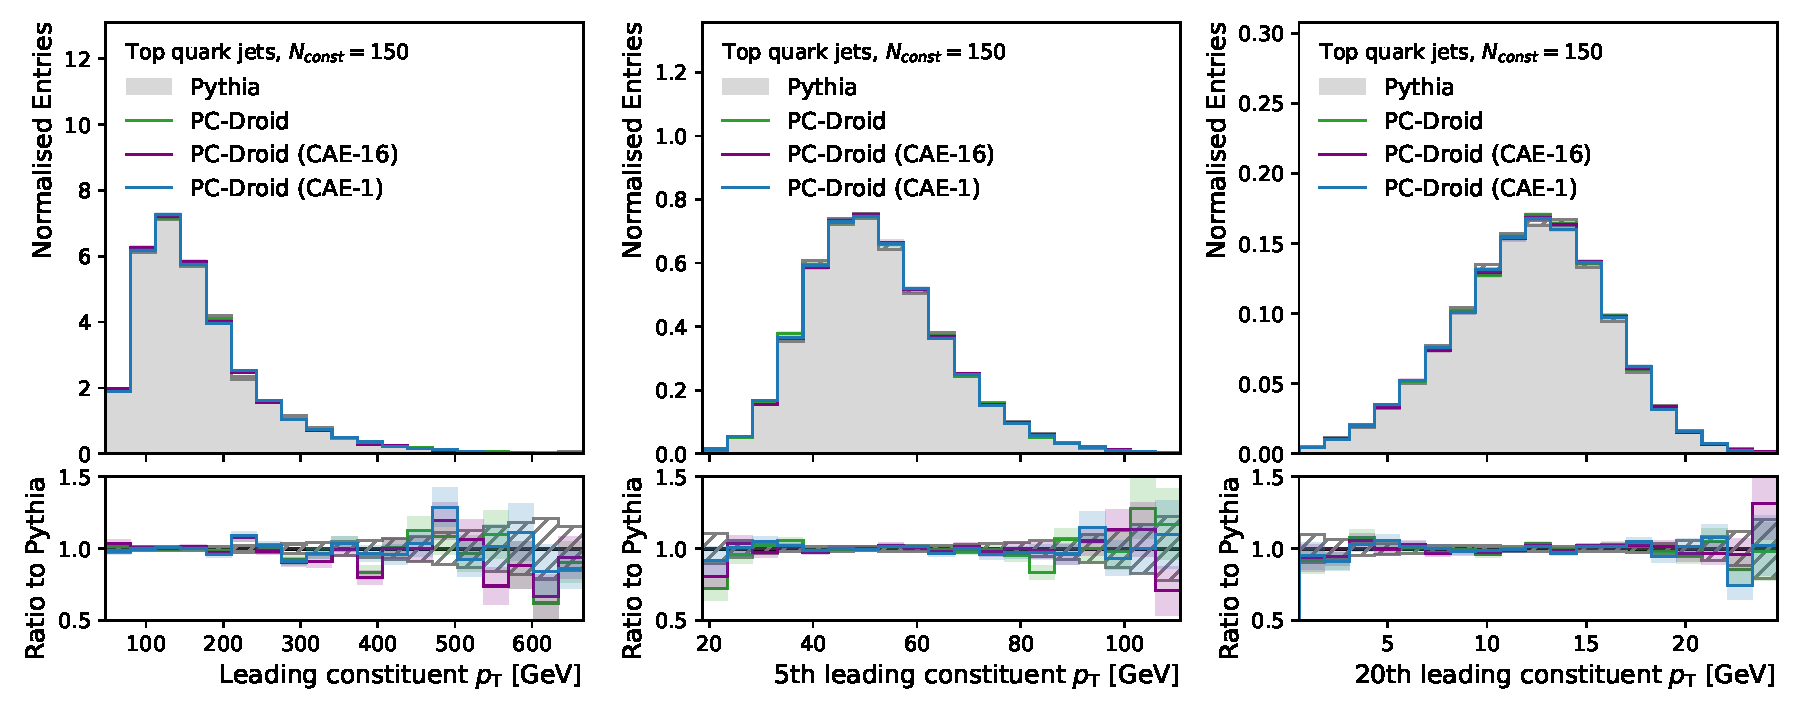
\includegraphics[width=0.99\textwidth]{Figures/jet_generation/droid/150/csts/t/100/t_leading_constituents.pdf}
    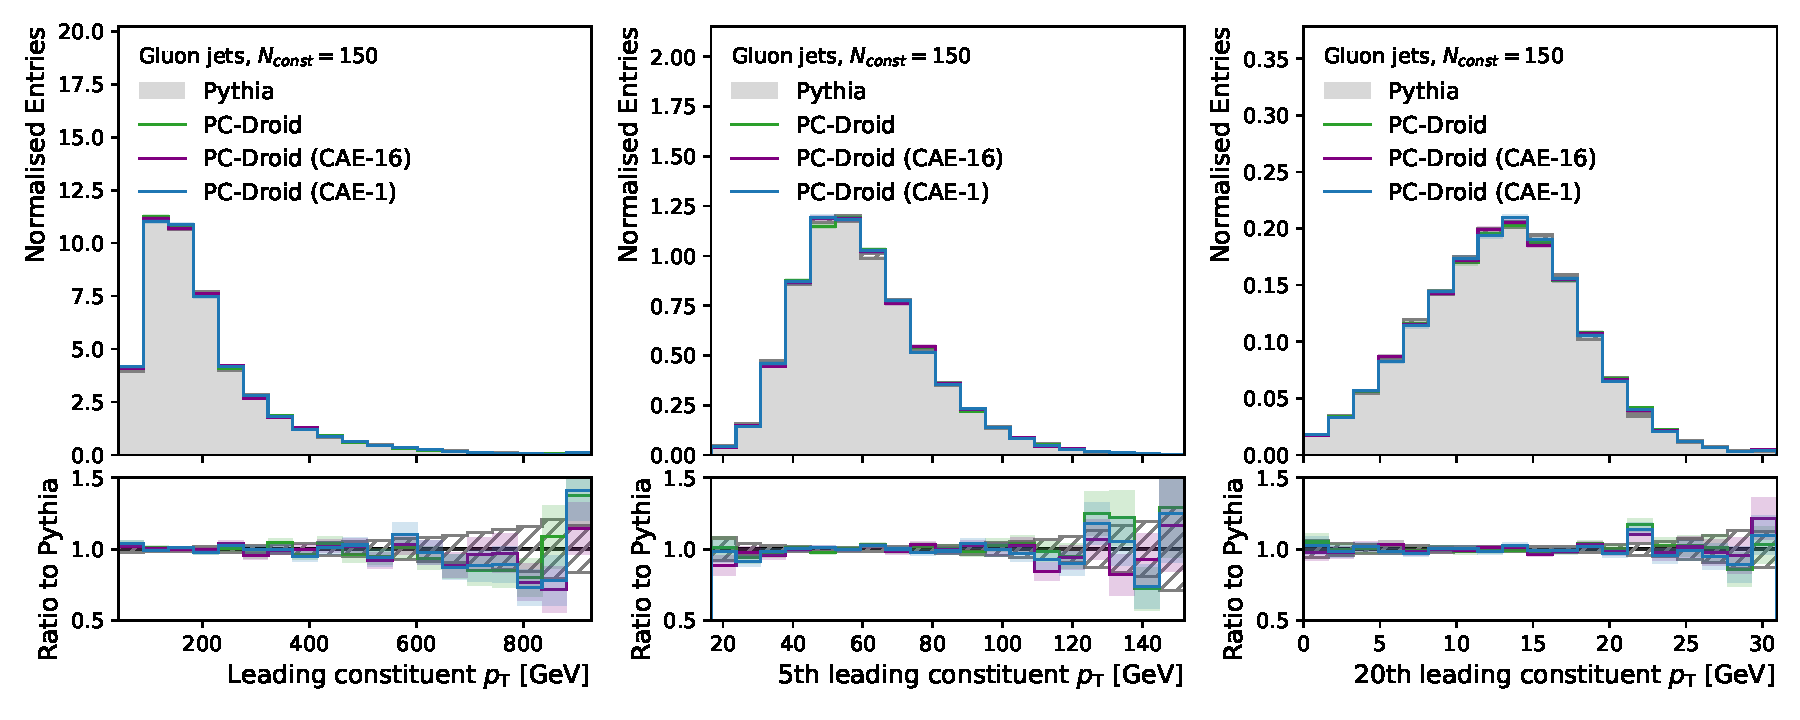
\includegraphics[width=0.99\textwidth]{Figures/jet_generation/droid/150/csts/g/100/g_leading_constituents.pdf}
    \caption{Comparison of \pt distributions of the leading, fifth leading, and twentieth leading constituents of the generated top and gluon jets with up to 150 constituents.
    }
    \label{fig:const-pt_dist-150}
\end{figure}

\begin{figure}[tb]
    \centering
    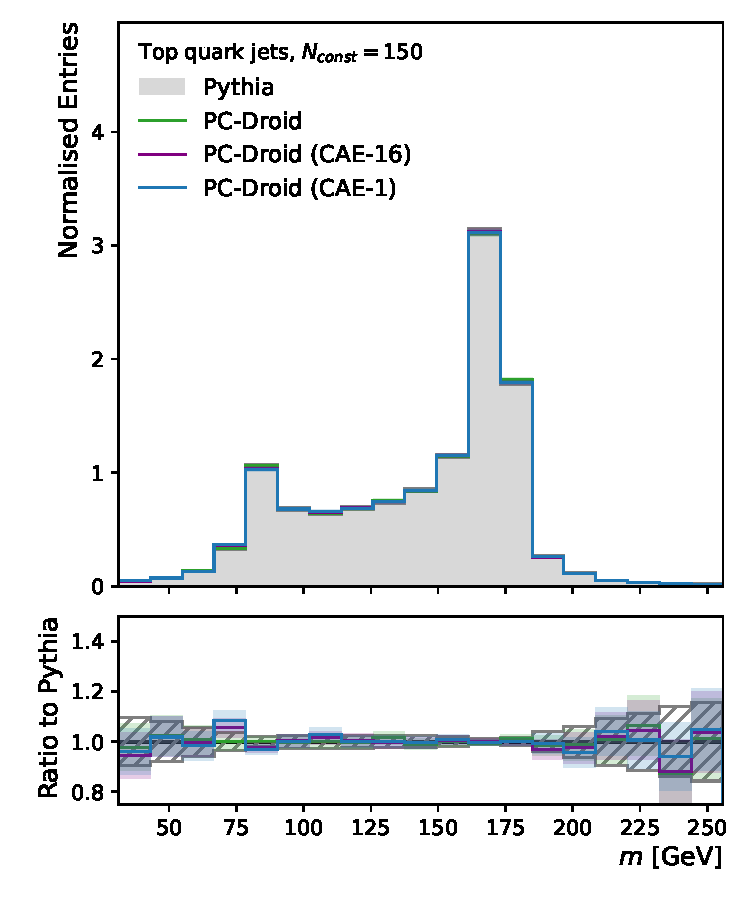
\includegraphics[width=0.33\textwidth]{Figures/jet_generation/droid/150/hlvs/t/100/mass.pdf}
    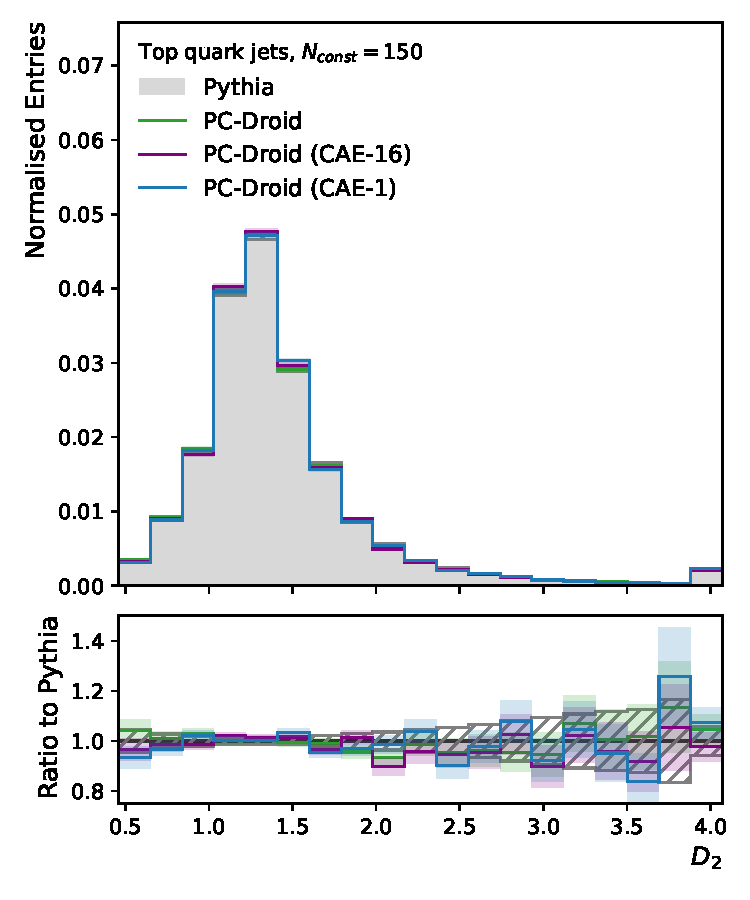
\includegraphics[width=0.33\textwidth]{Figures/jet_generation/droid/150/hlvs/t/100/d2.pdf} \\
    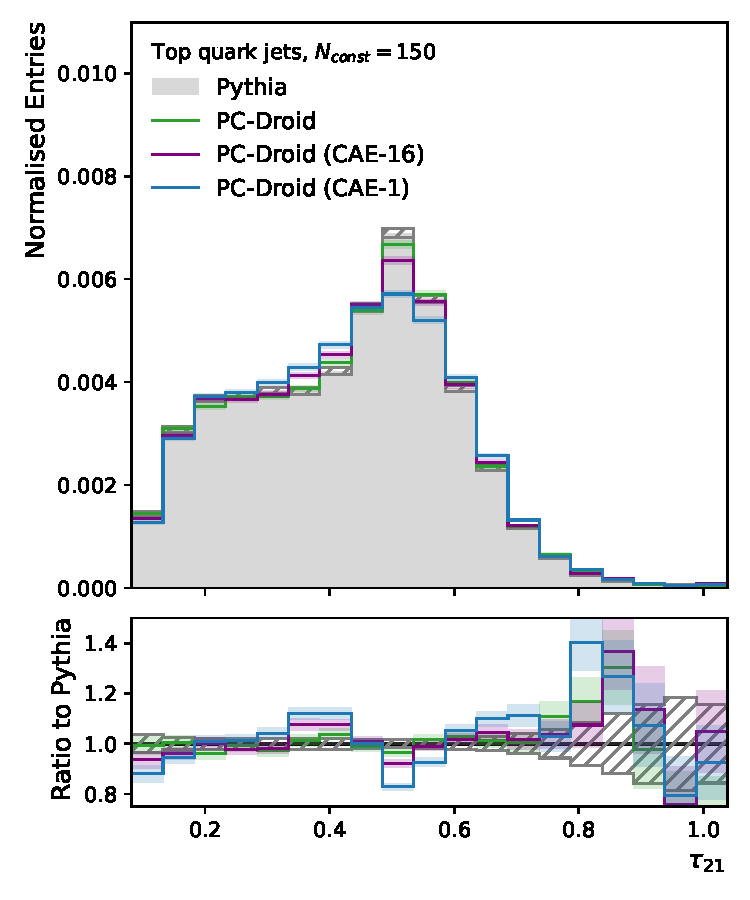
\includegraphics[width=0.33\textwidth]{Figures/jet_generation/droid/150/hlvs/t/100/tau_21.pdf}
    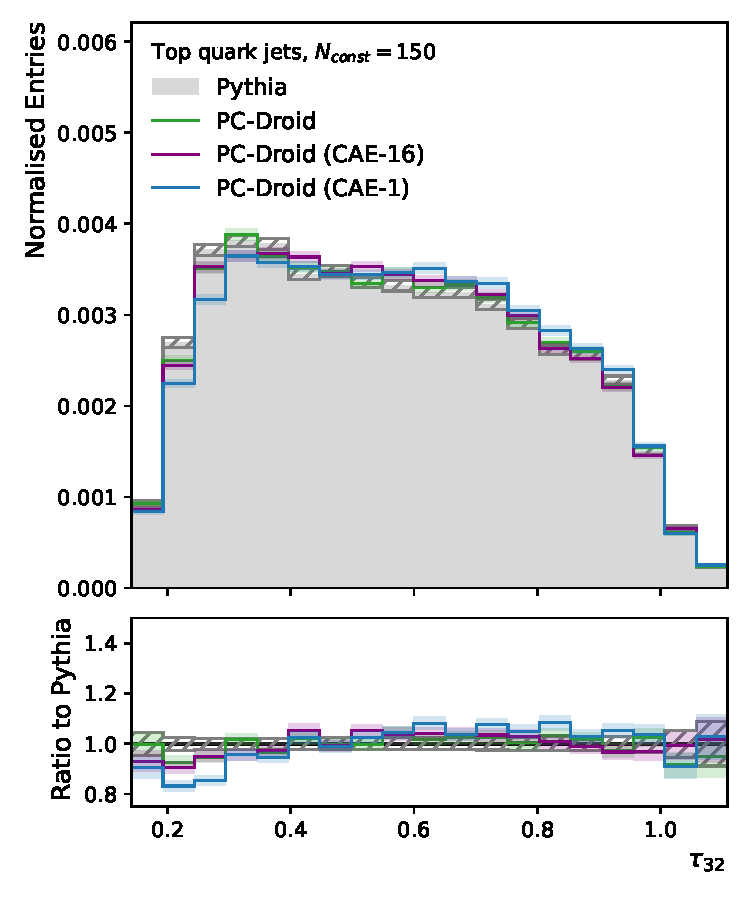
\includegraphics[width=0.33\textwidth]{Figures/jet_generation/droid/150/hlvs/t/100/tau_32.pdf}
    \caption{
        Comparison of the standard transformer based \pcdroid and the cross-attention encoder (CAE) variants using the generated mass and substructure marginals of top jets with up to 150 constituents.
    }
    \label{fig:hlvs-150-marginals}
\end{figure}

\begin{figure}[tb]
    \centering
    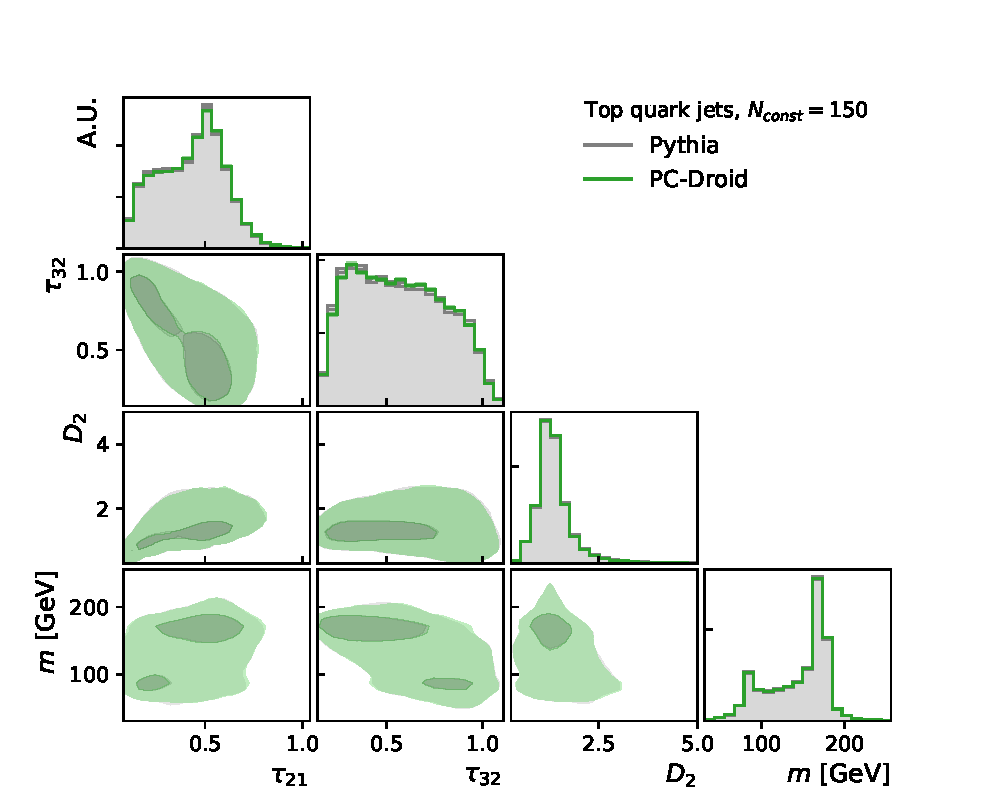
\includegraphics[width=0.49\textwidth]{Figures/jet_generation/droid/150/hlvs/t/100/hlv_corr_PC-Droid.pdf}
    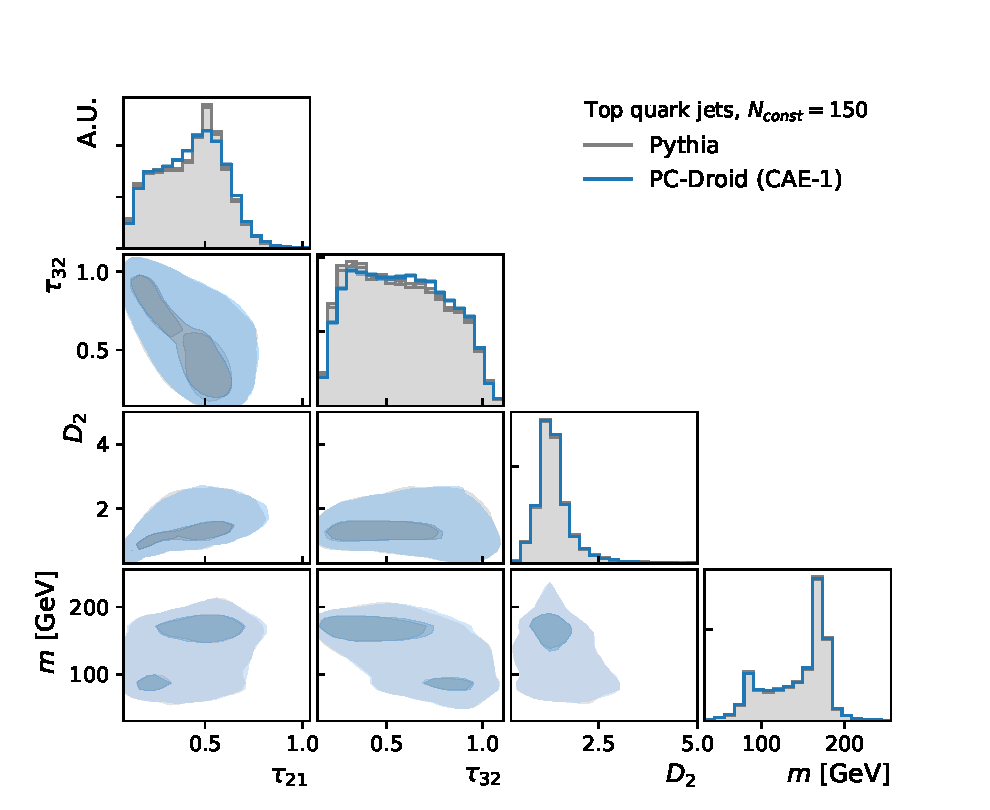
\includegraphics[width=0.49\textwidth]{Figures/jet_generation/droid/150/hlvs/t/100/hlv_corr_PC-DroidCAE1.pdf}
    \caption{
        Mass and substructure distributions of the generated top jets with up to 150 constituents.
        The diagonal consists of the marginals of the distributions and the off-diagonal elements contain the joint distributions.
    }
    \label{fig:hlvs-150}
\end{figure}

\begin{table}[tb]
    \centering
    \renewcommand{\arraystretch}{1.5}
    \caption{Comparison of generative models on top and gluon jets with up to 150 constituents. Lower is better. The FPND score is only defined for the first three classes and is sensitive only to the leading 30 constituents in \pt.}
    \label{tab:perf-150}
    \resizebox{\textwidth}{!}{%
        \begin{tabular}{llrrrrrrrc}
    \toprule
    Jet & Model             & NFE   & FPND            & $\mathrm{W_1^P}$ $(\times 10^{-4})$ & $\mathrm{W}_1^\mathrm{EFP}$ $(\times 10^{-6})$ & $\mathrm{W}_1^m$ $(\times 10^{-4})$ & $\mathrm{W}_1^{\tau_{21}}$ $(\times 10^{-3})$ & $\mathrm{W}_1^{\tau_{32}}$ $(\times 10^{-3})$ & $\mathrm{W}_1^{\Dtwo}$ $(\times 10^{-2})$ \\
    \midrule

    \multirow{10}{*}{Top}
        & \pythia           & $-$   & $0.01$          & $3.03 \pm 0.78$                     & $14.77 \pm 5.61$                               & $3.96 \pm 0.94$                     & $1.78 \pm 0.56$                               & $2.78 \pm 1.03$                               & $1.31 \pm 0.32$                           \\ \cline{2-10}
        & \pcdroid          & $100$ & $\mathbf{0.01}$ & $5.45 \pm 1.70$                     & $\mathbf{15.41 \pm 5.38}$                      & $\mathbf{3.60 \pm 1.20}$            & $\mathbf{2.87 \pm 1.20}$                      & $\mathbf{4.70 \pm 1.88}$                      & $\mathbf{1.15 \pm 0.30}$                  \\
        & \pcdroid (CAE-1)  & 100   & $0.06$          & $\mathbf{4.03 \pm 1.37}$            & $19.93 \pm 6.76$                               & $4.28 \pm 1.51$                     & $5.21 \pm 0.71$                               & $13.01 \pm 2.08$                              & $1.38 \pm 0.34$                           \\
        & \pcdroid (CAE-16) & 100   & $0.02$          & $5.40 \pm 1.43$                     & $17.17 \pm 5.85$                               & $4.63 \pm 1.28$                     & $3.22 \pm 0.61$                               & $5.94 \pm 1.55$                               & $1.31 \pm 0.28$                           \\
        & \pcdroid (CD1)    & $1$   & $0.13$          & $6.62 \pm 1.49$                     & $55.49 \pm 6.99$                               & $11.18 \pm 2.44$                    & $19.04 \pm 1.61$                              & $36.48 \pm 1.67$                              & $2.38 \pm 0.40$                           \\
        & \pcdroid (CD5)    & $5$   & $0.10$          & $6.78 \pm 1.76$                     & $54.25 \pm 5.27$                               & $9.24 \pm 1.53$                     & $7.53 \pm 0.79$                               & $22.98 \pm 1.58$                              & $1.31 \pm 0.30$                           \\
        & FPCD              & $512$ & $0.15$          & $4.36 \pm 1.28$                     & $26.11 \pm 6.30$                               & $6.44 \pm 2.57$                     & $6.30 \pm 0.81$                               & $9.91 \pm 1.39$                               & $1.47 \pm 0.36$                           \\
        & FPCD (PD1)        & $1$   & $0.53$          & $4.80 \pm 1.31$                     & $38.22 \pm 3.65$                               & $8.44 \pm 1.30$                     & $19.67 \pm 1.43$                              & $52.16 \pm 2.12$                              & $3.41 \pm 0.65$                           \\
        & EPiC-GAN          & $1$   & $0.95$          & $36.70 \pm 1.80$                    & $30.29 \pm 5.01$                               & $6.93 \pm 1.49$                     & $13.28 \pm 1.80$                              & $37.56 \pm 1.92$                              & $2.41 \pm 0.36$                           \\
    \midrule

    \multirow{10}{*}{Gluon}
        & \pythia           & $-$   & $0.01$          & $3.88 \pm 1.24$                     & $10.66 \pm 3.30$                               & $6.04 \pm 2.18$                     & $2.92 \pm 1.20$                               & $1.74 \pm 0.45$                               & $3.84 \pm 1.29$                           \\ \cline{2-10}
        & \pcdroid          & $100$ & $\mathbf{0.01}$ & $3.69 \pm 1.35$                     & $10.30 \pm 4.36$                               & $5.26 \pm 2.43$                     & $\mathbf{3.13 \pm 1.10}$                      & $\mathbf{2.24 \pm 0.93}$                      & $4.34 \pm 1.18$                           \\
        & \pcdroid (CAE-1)  & 100   & $\mathbf{0.01}$ & $\mathbf{3.38 \pm 1.10}$            & $11.84 \pm 4.15$                               & $\mathbf{4.62 \pm 1.29}$            & $4.07 \pm 1.30$                               & $2.41 \pm 0.75$                               & $\mathbf{3.27 \pm 1.39}$                  \\
        & \pcdroid (CAE-16) & 100   & $\mathbf{0.01}$ & $4.37 \pm 1.43$                     & $\mathbf{10.09 \pm 2.94}$                      & $5.04 \pm 1.77$                     & $3.22 \pm 1.06$                               & $\mathbf{2.24 \pm 0.72}$                      & $3.30 \pm 1.02$                           \\
        & \pcdroid (CD1)    & $1$   & $0.10$          & $6.54 \pm 1.81$                     & $21.55 \pm 6.13$                               & $5.55 \pm 2.76$                     & $15.33 \pm 2.58$                              & $10.73 \pm 0.80$                              & $4.52 \pm 1.12$                           \\
        & \pcdroid (CD5)    & $5$   & $0.06$          & $7.05 \pm 1.74$                     & $14.91 \pm 5.38$                               & $7.09 \pm 2.90$                     & $11.11 \pm 2.23$                              & $9.04 \pm 0.71$                               & $6.91 \pm 2.45$                           \\
        & FPCD              & $512$ & $0.03$          & $5.14 \pm 1.45$                     & $14.59 \pm 4.37$                               & $5.51 \pm 2.53$                     & $5.64 \pm 1.85$                               & $2.74 \pm 0.66$                               & $3.72 \pm 1.63$                           \\
        & FPCD (PD1)        & $1$   & $0.08$          & $5.53 \pm 1.24$                     & $18.83 \pm 5.71$                               & $6.83 \pm 1.61$                     & $19.36 \pm 2.45$                              & $10.97 \pm 1.03$                              & $7.83 \pm 1.60$                           \\
        & EPiC-GAN          & $1$   & $0.54$          & $32.22 \pm 1.83$                    & $12.72 \pm 4.14$                               & $5.00 \pm 1.47$                     & $15.49 \pm 2.14$                              & $13.32 \pm 1.08$                              & $4.03 \pm 1.15$                           \\
    \midrule

    \multirow{10}{*}{Quark}
        & \pythia           & $-$   & $0.01$          & $4.87 \pm 1.98$                     & $7.38 \pm 2.13$                                & $4.54 \pm 1.69$                     & $2.79 \pm 0.89$                               & $1.92 \pm 0.60$                               & $5.34 \pm 1.69$                           \\ \cline{2-10}
        & \pcdroid          & $100$ & $\mathbf{0.01}$ & $5.96 \pm 1.76$                     & $6.13 \pm 1.91$                                & $4.42 \pm 1.86$                     & $3.58 \pm 0.96$                               & $\mathbf{1.88 \pm 0.62}$                      & $\mathbf{6.42 \pm 2.68}$                  \\
        & \pcdroid (CAE-1)  & 100   & $\mathbf{0.01}$ & $\mathbf{4.55 \pm 1.03}$            & $6.04 \pm 1.86$                                & $\mathbf{3.88 \pm 1.53}$            & $4.02 \pm 1.35$                               & $2.07 \pm 0.51$                               & $6.45 \pm 1.35$                           \\
        & \pcdroid (CAE-16) & 100   & $0.02$          & $5.93 \pm 2.33$                     & $\mathbf{5.54 \pm 1.63}$                       & $4.82 \pm 1.56$                     & $\mathbf{3.52 \pm 0.91}$                      & $2.40 \pm 0.66$                               & $7.01 \pm 3.17$                           \\
        & \pcdroid (CD1)    & $1$   & $0.27$          & $7.74 \pm 2.21$                     & $9.90 \pm 2.69$                                & $6.50 \pm 1.87$                     & $13.56 \pm 1.89$                              & $9.22 \pm 0.60$                               & $24.58 \pm 2.17$                          \\
        & \pcdroid (CD5)    & $5$   & $0.15$          & $9.87 \pm 2.07$                     & $7.87 \pm 2.19$                                & $4.14 \pm 1.54$                     & $12.32 \pm 1.65$                              & $6.41 \pm 0.71$                               & $15.73 \pm 2.28$                          \\
        & FPCD              & $512$ & $0.03$          & $5.32 \pm 1.86$                     & $5.99 \pm 1.81$                                & $7.28 \pm 2.12$                     & $3.71 \pm 1.10$                               & $3.36 \pm 0.75$                               & $6.72 \pm 2.39$                           \\
        & FPCD (PD1)        & $1$   & $0.09$          & $6.39 \pm 1.94$                     & $7.24 \pm 2.14$                                & $7.43 \pm 2.84$                     & $17.58 \pm 1.75$                              & $9.40 \pm 0.98$                               & $18.71 \pm 2.52$                          \\
        & EPiC-GAN          & $1$   & $0.17$          & $39.69 \pm 2.67$                    & $8.19 \pm 3.06$                                & $5.25 \pm 1.78$                     & $13.00 \pm 1.85$                              & $10.35 \pm 0.89$                              & $26.65 \pm 3.21$                          \\
    \midrule

    \multirow{9}{*}{W Boson}
        & \pythia           & $-$   & $-$             & $3.86 \pm 1.16$                     & $1.87 \pm 0.51$                                & $1.73 \pm 0.47$                     & $2.79 \pm 0.83$                               & $3.19 \pm 1.31$                               & $2.95 \pm 1.21$                           \\ \cline{2-10}
        & \pcdroid          & $100$ & $-$             & $\mathbf{3.32 \pm 0.98}$            & $\mathbf{1.49 \pm 0.38}$                       & $\mathbf{1.72 \pm 0.75}$            & $3.33 \pm 1.12$                               & $\mathbf{2.14 \pm 0.61}$                      & $\mathbf{2.73 \pm 0.99}$                  \\
        & \pcdroid (CAE-1)  & 100   & $-$             & $3.79 \pm 1.12$                     & $1.58 \pm 0.48$                                & $2.18 \pm 0.51$                     & $3.00 \pm 1.08$                               & $3.59 \pm 1.27$                               & $2.75 \pm 0.78$                           \\
        & \pcdroid (CAE-16) & 100   & $-$             & $3.93 \pm 1.03$                     & $1.82 \pm 0.49$                                & $2.04 \pm 0.56$                     & $\mathbf{2.81 \pm 0.83}$                      & $2.62 \pm 1.09$                               & $3.21 \pm 1.45$                           \\
        & \pcdroid (CD1)    & $1$   & $-$             & $5.06 \pm 1.16$                     & $6.47 \pm 0.89$                                & $12.80 \pm 0.93$                    & $26.98 \pm 1.57$                              & $10.64 \pm 0.73$                              & $6.42 \pm 0.74$                           \\
        & \pcdroid (CD5)    & $5$   & $-$             & $6.25 \pm 1.07$                     & $4.40 \pm 0.62$                                & $8.28 \pm 0.43$                     & $8.07 \pm 1.48$                               & $13.30 \pm 1.44$                              & $3.94 \pm 1.20$                           \\
        & FPCD              & $512$ & $-$             & $3.53 \pm 1.06$                     & $2.02 \pm 0.58$                                & $2.97 \pm 0.41$                     & $2.86 \pm 0.91$                               & $3.91 \pm 0.84$                               & $2.92 \pm 0.86$                           \\
        & FPCD (PD1)        & $1$   & $-$             & $4.32 \pm 1.40$                     & $4.00 \pm 0.57$                                & $9.07 \pm 0.51$                     & $20.78 \pm 1.48$                              & $7.90 \pm 0.45$                               & $7.31 \pm 1.22$                           \\
    \midrule

    \multirow{9}{*}{Z Boson}
        & \pythia           & $-$   & $-$             & $4.12 \pm 1.57$                     & $2.10 \pm 0.54$                                & $2.19 \pm 0.77$                     & $3.10 \pm 1.49$                               & $2.00 \pm 0.59$                               & $3.42 \pm 0.94$                           \\ \cline{2-10}
        & \pcdroid          & $100$ & $-$             & $3.90 \pm 1.32$                     & $\mathbf{2.01 \pm 0.67}$                       & $1.95 \pm 0.52$                     & $\mathbf{2.71 \pm 0.99}$                      & $\mathbf{2.22 \pm 0.62}$                      & $3.22 \pm 0.95$                           \\
        & \pcdroid (CAE-1)  & 100   & $-$             & $\mathbf{3.65 \pm 1.14}$            & $2.04 \pm 0.68$                                & $2.24 \pm 0.58$                     & $3.43 \pm 1.02$                               & $4.16 \pm 1.13$                               & $\mathbf{2.43 \pm 0.58}$                  \\
        & \pcdroid (CAE-16) & 100   & $-$             & $3.87 \pm 1.15$                     & $2.19 \pm 0.53$                                & $\mathbf{1.90 \pm 0.73}$            & $3.28 \pm 1.18$                               & $2.58 \pm 1.04$                               & $3.08 \pm 0.92$                           \\
        & \pcdroid (CD1)    & $1$   & $-$             & $5.04 \pm 0.94$                     & $6.57 \pm 0.73$                                & $12.20 \pm 0.53$                    & $22.78 \pm 2.07$                              & $9.32 \pm 0.67$                               & $6.12 \pm 1.09$                           \\
        & \pcdroid (CD5)    & $5$   & $-$             & $5.41 \pm 1.21$                     & $6.16 \pm 0.74$                                & $7.99 \pm 0.45$                     & $6.39 \pm 1.28$                               & $15.49 \pm 1.23$                              & $3.40 \pm 0.88$                           \\
        & FPCD              & $512$ & $-$             & $4.66 \pm 1.35$                     & $2.59 \pm 0.61$                                & $2.97 \pm 0.53$                     & $3.90 \pm 1.35$                               & $4.26 \pm 1.14$                               & $3.05 \pm 0.73$                           \\
        & FPCD (PD1)        & $1$   & $-$             & $4.72 \pm 1.26$                     & $5.91 \pm 0.75$                                & $9.63 \pm 0.93$                     & $23.70 \pm 1.76$                              & $8.52 \pm 1.08$                               & $6.55 \pm 1.04$                           \\
    \bottomrule
\end{tabular}

    }
\end{table}

\FloatBarrier

\subsubsection{Conditional Adherence}

It is important to test the claim that \pcdroid is actually a contidiional generative model.
The difference between the generated point cloud kinematics and the target conditions for mass and \pt is examined, as shown in Figure \ref{fig:obedience}.

The exact jet kinematics from the simulation are used for the \textit{conditional kinematics}, while the \textit{point cloud kinematics} are recalculated from the trimmed jet constituents.
These different approaches result in minor discrepancies between the variables, even for the \pythia dataset.
The original jets may have had more than 150 constituents when the kinematics were calculated, causing a negative shift in mass and \pt.

In the mass plot in \Cref{fig:obedience}, \pcdroid displays a nearly identical spread to \pythia.
For \pt, there is slightly more variation with higher residual magnitudes, but \pcdroid remains within $0.4\%$ of the target

\begin{figure}[htpb]
    \centering
    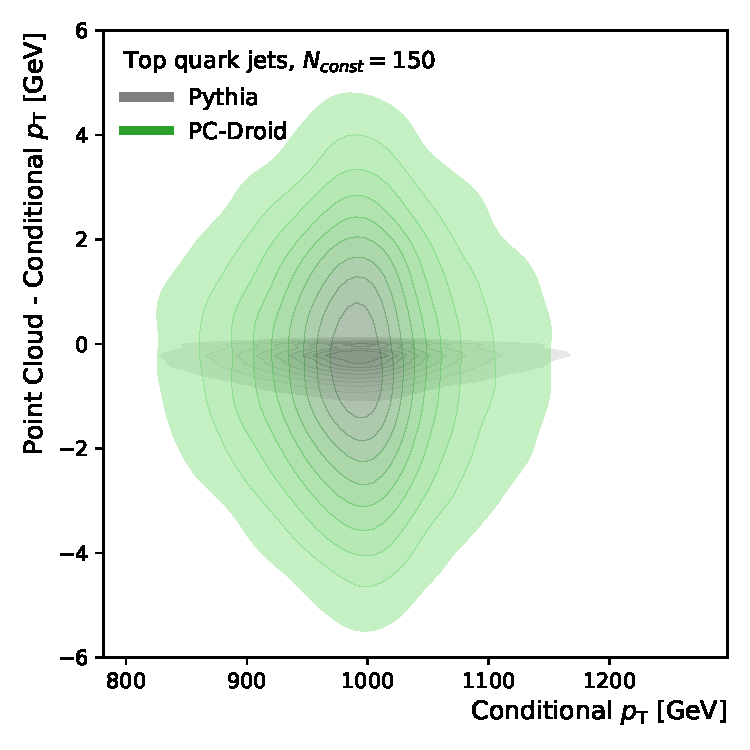
\includegraphics[width=0.32\textwidth]{Figures/jet_generation/droid/150/obedience/t/100/t_pt_PC-Droid_resid.pdf}
    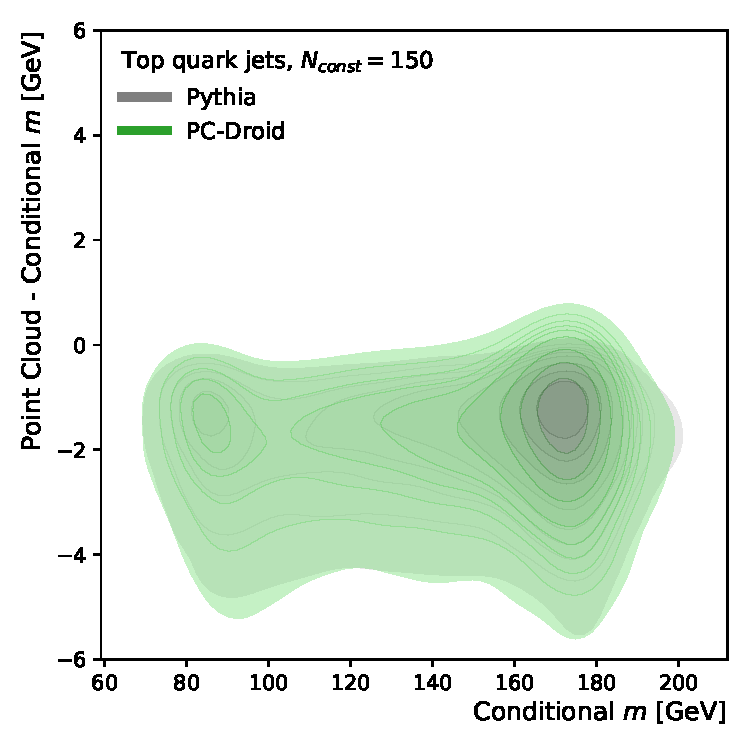
\includegraphics[width=0.32\textwidth]{Figures/jet_generation/droid/150/obedience/t/100/t_mass_PC-Droid_resid.pdf}
    \caption{The correlation between the conditional and point cloud kinematics on top jets with up to 150 constituents. The $y$-axis, shows the difference between the two variables.}
    \label{fig:obedience}
\end{figure}

\subsubsection{Consistency Distillation}

Diffusion models inherently present a trade-off between the number of iterations during generation and the quality of the final sample.
Consistency models add another dimension to this trade-off by enabling the production of reasonable samples in as few as one iteration step, significantly outperforming diffusion models when highly constrained by time.

A consistency model is trained using the TE-based \pcdroid as the teacher
The same training configuration as the original paper by \textcite{ConsistencyModels} is adopted, with one modification: instead of using the Heun integration solver to select adjacent points of the ODE, DPM-Solver-2 yields improved performance.

During generation, reasonable performance is achieved with just a single network pass, and performance plateaus after five steps.
\Cref{fig:cd-150} compares the substructure variables for jets produced using the CD model with one-step (CD1) and five-step (CD5) generation.
The top jet subjettiness ratios continue to be the most challenging to reproduce, especially for the one-step model.

\begin{figure}[htpb]
    \centering
    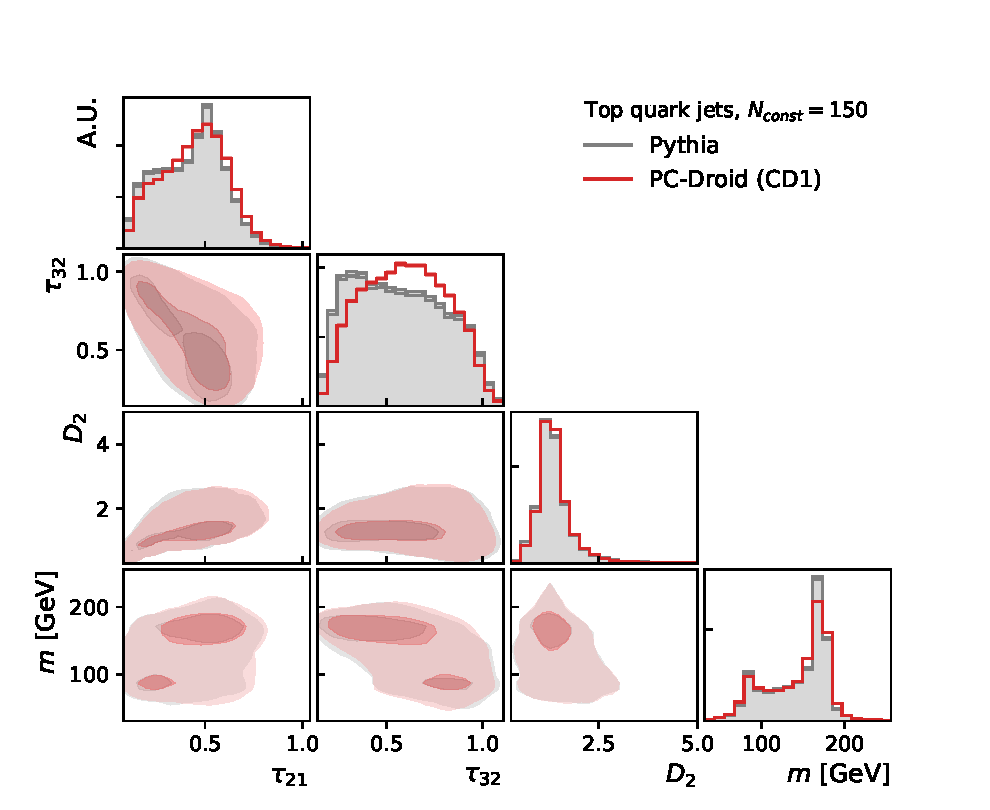
\includegraphics[width=0.49\textwidth]{Figures/jet_generation/droid/150/hlvs/t/100/hlv_corr_PC-DroidCD1.pdf}
    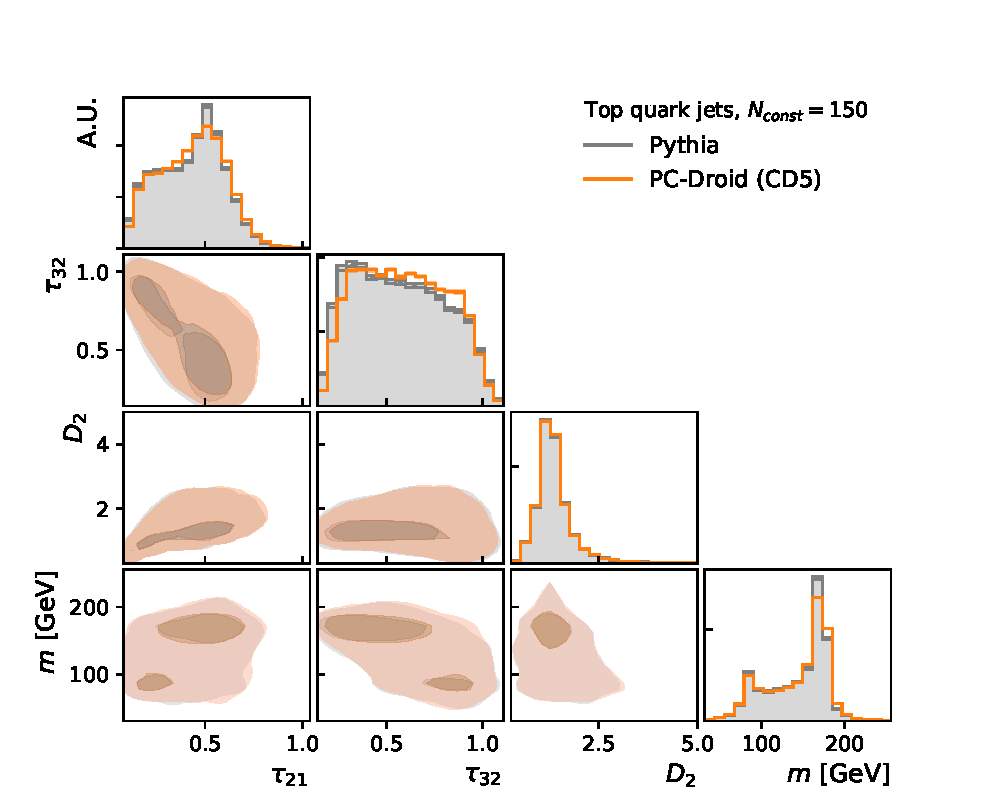
\includegraphics[width=0.49\textwidth]{Figures/jet_generation/droid/150/hlvs/t/100/hlv_corr_PC-DroidCD5.pdf}
    \caption{
        Mass and substructure distributions of the generated top jets with up to 150 constituents using the CD models.
        The diagonal consists of the marginals and the off-diagonal elements contain the joint distributions.
    }
    \label{fig:cd-150}
\end{figure}

\subsubsection{Modelling The Conditional Variables}

Utilizing normalizing flows provides flexibility to sample either the complete set of jet kinematics along with $N_{const}$ (Flow-$\p$) or just $N_{const}$ (Flow-$N$), both conditional on PID.
These flows are trained independently of \pcdroid, as this is an entirely orthogonal task.
The performance of Flow-$\p$ is showcased in \Cref{fig:unconditional-flows}, illustrating that the marginals and correlations of the conditioning variables are accurately modeled.

The conditional and unconditional models are evaluated using the full array of metrics in \Cref{tab:perf-150-unconditional}.
Here, \pcdroid denotes the conditional model, where $N_{const}$ and the jet kinematics are derived from the test set.
The other two rows represent scenarios where either flow is used to initially sample these variables before passing them to the diffusion model.
There is minimal difference in performance when shifting to unconditional generation.

\begin{figure}[b!]
    \centering
    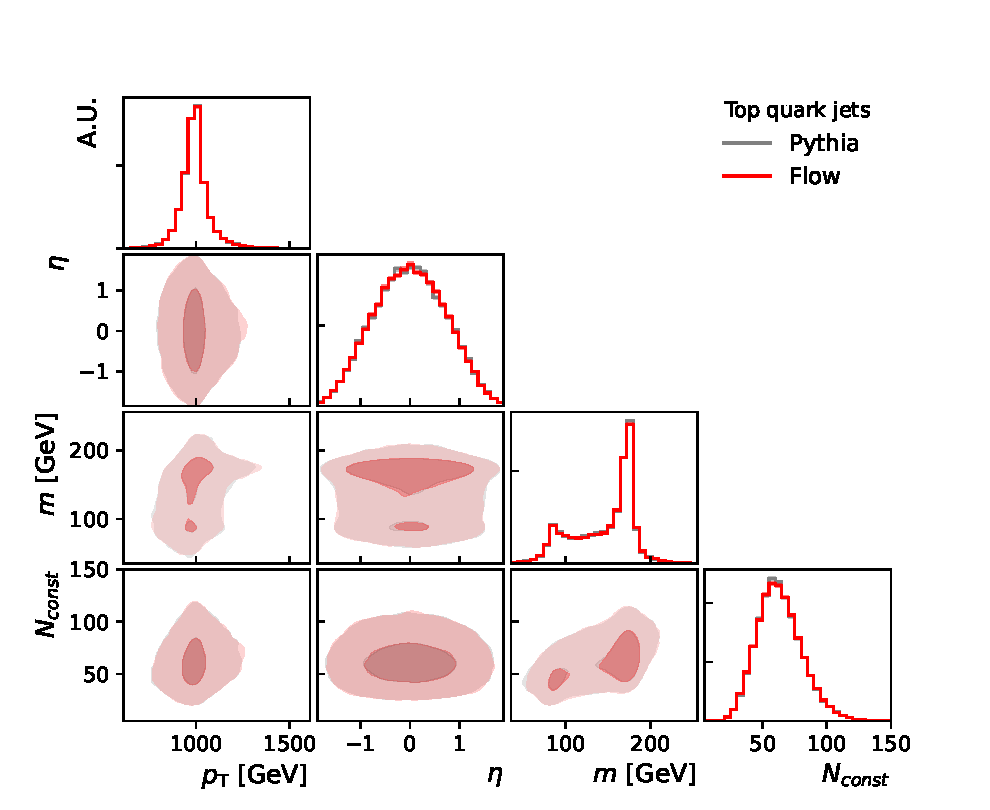
\includegraphics[width=0.49\linewidth]{Figures/jet_generation/droid/150/flow_quality_t.pdf}
    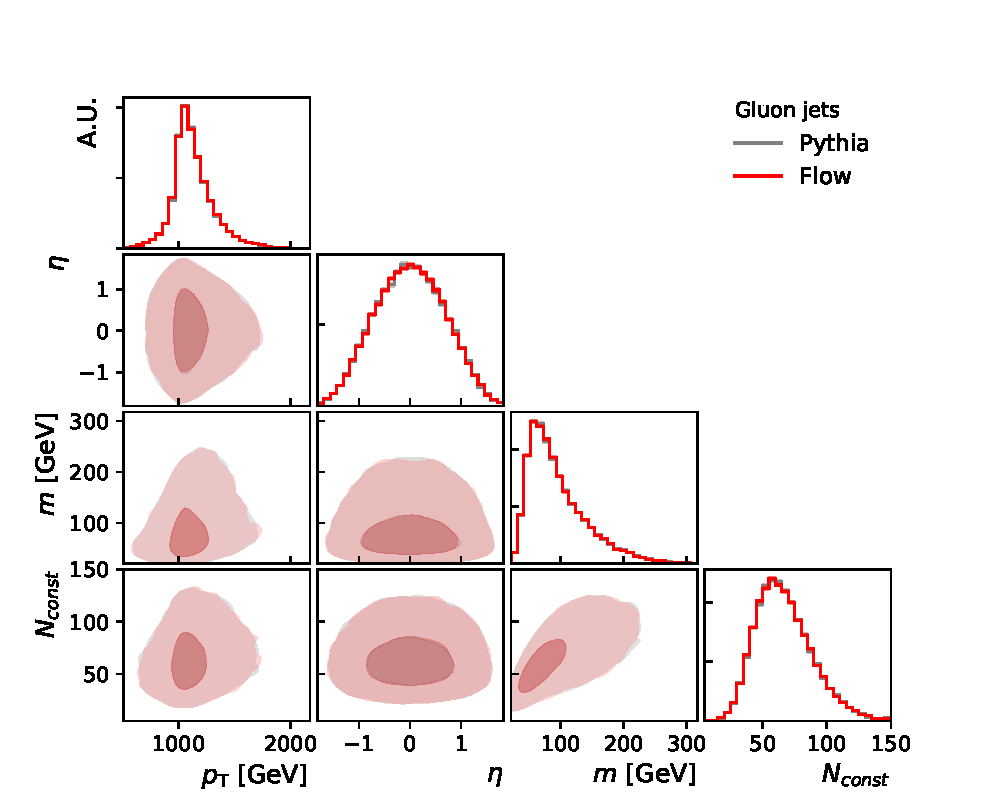
\includegraphics[width=0.49\linewidth]{Figures/jet_generation/droid/150/flow_quality_g.pdf}
    \caption{Marginals of the conditioning variables generated with Flow-$\p$ compared to \pythia for top and gluon jets with up to 150 constituents.
    }
    \label{fig:unconditional-flows}
\end{figure}

\begin{table}[tp]
    \centering
    \renewcommand{\arraystretch}{1.5}
    \caption{Comparison of conditional and unconditional models on jets with up to 150 constituents. The FPND score is only defined for the first three classes and is sensitive only to the leading 30 constituents in \pt.
    }
    \label{tab:perf-150-unconditional}
    \resizebox{\textwidth}{!}{%
        \begin{tabular}{llrrrrrrr}
    \toprule
    Jet & Model                & FPND            & $\mathrm{W_1^P}$ $(\times 10^{-4})$ & $\mathrm{W}_1^\mathrm{EFP}$ $(\times 10^{-6})$ & $\mathrm{W}_1^m$ $(\times 10^{-4})$ & $\mathrm{W}_1^{\tau_{21}}$ $(\times 10^{-3})$ & $\mathrm{W}_1^{\tau_{32}}$ $(\times 10^{-3})$ & $\mathrm{W}_1^{\Dtwo}$ $(\times 10^{-2})$ \\
    \midrule

    \multirow{4}{*}{Top}
        & \pythia              & $0.01$          & $3.03 \pm 0.78$                     & $14.77 \pm 5.61$                               & $3.96 \pm 0.94$                     & $1.78 \pm 0.56$                               & $2.78 \pm 1.03$                               & $1.31 \pm 0.32$                           \\ \cline{2-9}
        & \pcdroid             & $\mathbf{0.01}$ & $5.45 \pm 1.70$                     & $15.41 \pm 5.38$                               & $\mathbf{3.60 \pm 1.20}$            & $2.87 \pm 1.20$                               & $4.70 \pm 1.88$                               & $\mathbf{1.15 \pm 0.30}$                  \\
        & \pcdroid (Flow-$\p$) & $0.02$          & $4.95 \pm 1.34$                     & $17.97 \pm 4.44$                               & $4.84 \pm 1.18$                     & $3.40 \pm 1.29$                               & $5.35 \pm 1.33$                               & $1.23 \pm 0.36$                           \\
        & \pcdroid (Flow-$N$)  & $\mathbf{0.01}$ & $\mathbf{4.89 \pm 1.47}$            & $\mathbf{14.14 \pm 3.93}$                      & $3.91 \pm 1.35$                     & $3.39 \pm 1.28$                               & $5.28 \pm 1.33$                               & $1.38 \pm 0.27$                           \\
    \midrule

    \multirow{4}{*}{Gluon}
        & \pythia              & $0.01$          & $3.88 \pm 1.24$                     & $10.66 \pm 3.30$                               & $6.04 \pm 2.18$                     & $2.92 \pm 1.20$                               & $1.74 \pm 0.45$                               & $3.84 \pm 1.29$                           \\ \cline{2-9}
        & \pcdroid             & $\mathbf{0.01}$ & $3.69 \pm 1.35$                     & $10.30 \pm 4.36$                               & $5.26 \pm 2.43$                     & $3.13 \pm 1.10$                               & $2.24 \pm 0.93$                               & $4.34 \pm 1.18$                           \\
        & \pcdroid (Flow-$\p$) & $\mathbf{0.01}$ & $\mathbf{3.63 \pm 1.56}$            & $10.63 \pm 2.07$                               & $6.10 \pm 3.02$                     & $3.43 \pm 1.19$                               & $2.24 \pm 0.91$                               & $4.50 \pm 1.82$                           \\
        & \pcdroid (Flow-$N$)  & $0.02$          & $4.01 \pm 1.22$                     & $\mathbf{9.74 \pm 2.53}$                       & $\mathbf{4.90 \pm 1.54}$            & $3.40 \pm 1.21$                               & $\mathbf{2.20 \pm 0.90}$                      & $\mathbf{3.13 \pm 0.83}$                  \\
    \midrule

    \multirow{4}{*}{Quark}
        & \pythia              & $0.01$          & $4.87 \pm 1.98$                     & $7.38 \pm 2.13$                                & $4.54 \pm 1.69$                     & $2.79 \pm 0.89$                               & $1.92 \pm 0.60$                               & $5.34 \pm 1.69$                           \\ \cline{2-9}
        & \pcdroid             & $\mathbf{0.01}$ & $5.96 \pm 1.76$                     & $\mathbf{6.13 \pm 1.91}$                       & $4.42 \pm 1.86$                     & $3.58 \pm 0.96$                               & $1.88 \pm 0.62$                               & $6.42 \pm 2.68$                           \\
        & \pcdroid (Flow-$\p$) & $\mathbf{0.01}$ & $7.18 \pm 2.33$                     & $6.46 \pm 1.42$                                & $4.83 \pm 1.41$                     & $2.95 \pm 1.04$                               & $2.26 \pm 0.79$                               & $\mathbf{5.70 \pm 2.00}$                  \\
        & \pcdroid (Flow-$N$)  & $\mathbf{0.01}$ & $\mathbf{5.52 \pm 1.86}$            & $6.40 \pm 1.82$                                & $\mathbf{4.19 \pm 1.07}$            & $\mathbf{2.92 \pm 1.05}$                      & $2.26 \pm 0.78$                               & $6.86 \pm 2.07$                           \\
    \midrule

    \multirow{4}{*}{W Boson}
        & \pythia              & $-$             & $3.86 \pm 1.16$                     & $1.87 \pm 0.51$                                & $1.73 \pm 0.47$                     & $2.79 \pm 0.83$                               & $3.19 \pm 1.31$                               & $2.95 \pm 1.21$                           \\ \cline{2-9}
        & \pcdroid             & $-$             & $\mathbf{3.32 \pm 0.98}$            & $\mathbf{1.49 \pm 0.38}$                       & $1.72 \pm 0.75$                     & $3.33 \pm 1.12$                               & $2.14 \pm 0.61$                               & $\mathbf{2.73 \pm 0.99}$                  \\
        & \pcdroid (Flow-$\p$) & $-$             & $3.77 \pm 1.08$                     & $2.07 \pm 0.50$                                & $2.27 \pm 0.58$                     & $3.02 \pm 1.02$                               & $3.27 \pm 1.04$                               & $2.81 \pm 0.93$                           \\
        & \pcdroid (Flow-$N$)  & $-$             & $3.62 \pm 0.98$                     & $1.82 \pm 0.44$                                & $\mathbf{1.70 \pm 0.58}$            & $3.08 \pm 1.01$                               & $3.31 \pm 1.06$                               & $2.82 \pm 0.89$                           \\
    \midrule


    \multirow{4}{*}{Z Boson}
        & \pythia              & $-$             & $4.12 \pm 1.57$                     & $2.10 \pm 0.54$                                & $2.19 \pm 0.77$                     & $3.10 \pm 1.49$                               & $2.00 \pm 0.59$                               & $3.42 \pm 0.94$                           \\ \cline{2-9}
        & \pcdroid             & $-$             & $3.90 \pm 1.32$                     & $2.01 \pm 0.67$                                & $1.95 \pm 0.52$                     & $2.71 \pm 0.99$                               & $2.22 \pm 0.62$                               & $3.22 \pm 0.95$                           \\
        & \pcdroid (Flow-$\p$) & $-$             & $\mathbf{3.62 \pm 1.07}$            & $1.86 \pm 0.39$                                & $1.95 \pm 0.69$                     & $3.03 \pm 1.05$                               & $2.34 \pm 0.67$                               & $2.72 \pm 0.71$                           \\
        & \pcdroid (Flow-$N$)  & $-$             & $4.46 \pm 1.48$                     & $\mathbf{1.81 \pm 0.51}$                       & $\mathbf{1.70 \pm 0.66}$            & $3.01 \pm 1.06$                               & $2.31 \pm 0.67$                               & $\mathbf{2.56 \pm 0.80}$                  \\
    \bottomrule
\end{tabular}

    }
\end{table}

\FloatBarrier

\subsubsection{Timing Studies}

\Cref{fig:timing} illustrates three key metrics for all models as a function of the generation time required to produce top jets with 150 constituents on identical hardware.
All times are derived from the average of ten runs, each generating a batch of 512 jets using an NVIDIA GeForce 3080.
All scores are defined as their ratio to ideal performance, as defined by the \pythia datasets.

The fastest of the new models, CD1, requires three times the generation time of EPiC-GAN.
It induces a slight shift in the jet mass while improving the FPND score considerably.
It is nearly 30\% faster than one step FPCD (PD1) and shows markedly improved performance, especially in FPND.
The $\tau_{32}$ scores of these models are comparable.
CD5, although five times slower than the one-shot generation, improves all metrics across the board.
CAE-1 further enhances all metrics, particularly $\mathrm{W}_1^m$.
By increasing the number of global tokens to 16, a 50\% increase in generation time is observed, but a significant improvement in both FPND and $\mathrm{W}1^{\tau{32}}$ is achieved.
The full \pcdroid model, while approximately 250 times slower than EPiC-GAN, achieves nearly ideal performance in all metrics except $\mathrm{W}1^{\tau{32}}$, and is still around 4 times faster than the \pythia simulation.

\begin{figure}[htbp]
    \centering
    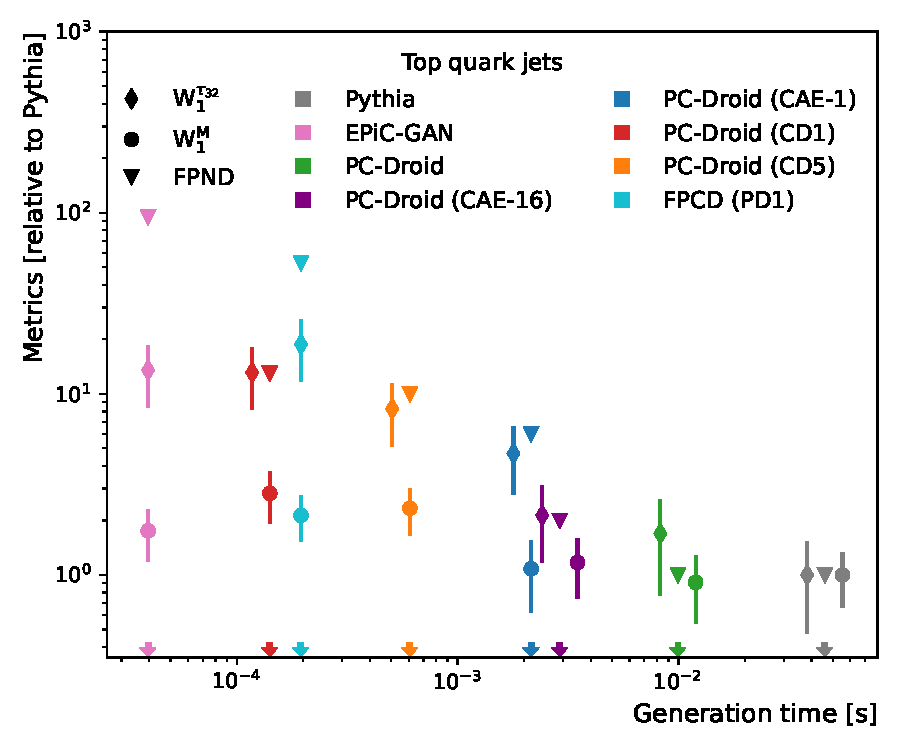
\includegraphics[width=0.5\textwidth]{Figures/jet_generation/droid/150/metrics_vs_times/t/t_metrics_vs_times.pdf}
    \caption{Performance as a ratio to \pythia as a function of the required generation time for a top jet with up to 150 constituents. The time for \pythia is taken from Ref.~\cite{MPGAN}.}
    \label{fig:timing}
\end{figure}

\subsection{Diffusion with EPiC Layers}

Collaboration with the research group responsible for the EPiC-GAN model led to the integration of the diffusion model with their EPiC layers~\cite{EpicJedi}.
In this study, experiments using the conditional flow matchinng (CFM) framework to describe the diffusion process proved significantly more efficient than the SM-TI framework employed in \pcjedi.
This research, conducted concurrently with the development of \pcdroid, is only compared to the \pcjedi model.

Utilizing these layers achieves approximately a seven-fold increase in generation speed over the transformer.
The resulting performance and generation time are comparable to the CAE-1 model from \pcdroid.
Once again, the subjettiness ratios remain particularly challenging to model for top jets, as illustrated in \Cref{fig:epic-diffusion}.

\begin{figure}[tb]
    \centering
    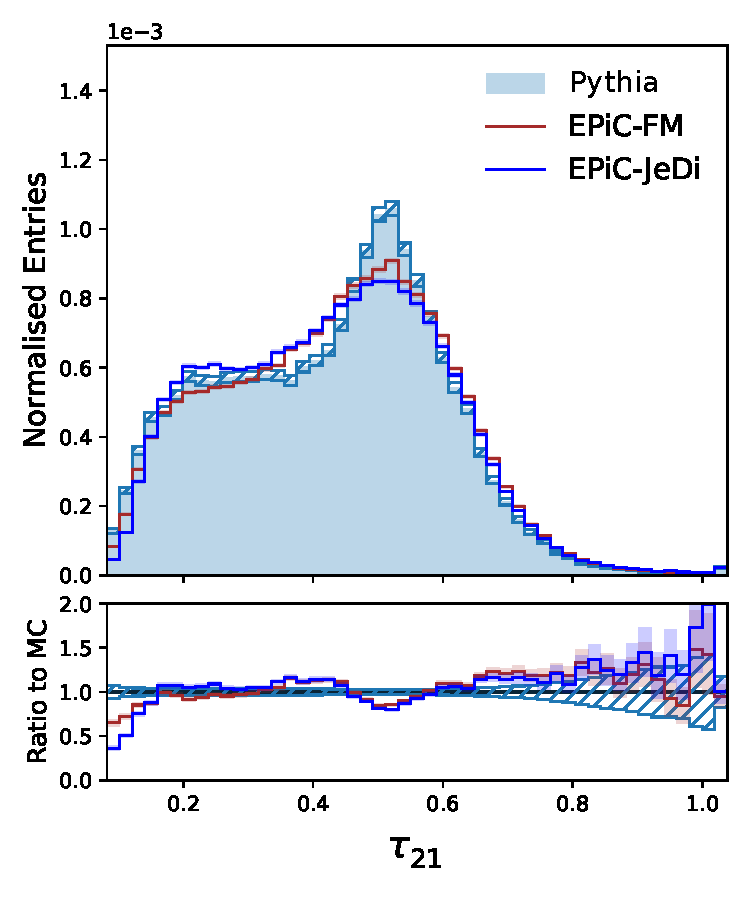
\includegraphics[width=0.33\textwidth]{Figures/jet_generation/t_tau21.pdf}
    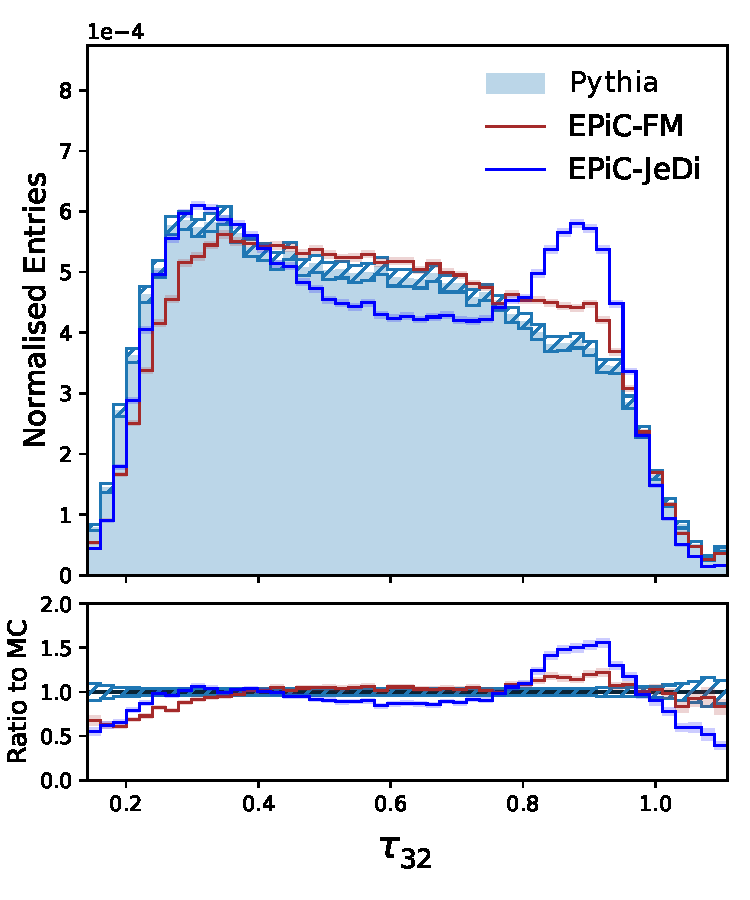
\includegraphics[width=0.33\textwidth]{Figures/jet_generation/t_tau32.pdf}
    \caption{
        Comparison between generative models using EPiC layers using the diffusion framework from \pcjedi verses the CFM framework.
    }
    \label{fig:epic-diffusion}
\end{figure}

\subsection{Conclusion}

The \pcdroid model, utilizing the EDM framework, outperforms \pcjedi and all other models in all metrics, especially in the subjettiness ratios of top jets.

Generative models employing diffusion processes present numerous points along the continuum between generation time and output quality.
Additional integration solvers enhance generation and consistency distillation, allowing for extremely fast generation, though with degraded quality.
The development of the CAE Block allows scaling to sets with higher multiplicities due to reduced computational overhead.

This framework represents a significant advancement in high-quality jet generation, now primed for applications in forward simulation and as a template construction tool for anomaly detection.

An area yet to be explored is the comparison between the CFM and EDM frameworks for this specific task.
While generative models for text-to-image generation have transitioned from EDM to CFM over the past year~\cite{SD3,flux2024github}, it remains uncertain if this trend applies to jet generation.

\section{Full Forward Simulation}

The full simulation pipeline for collider data consists of many subtasks.
It begins with event generation via matrix element calculation.
The decay of heavy quarks and massive bosons is then modelled, resulting in parton-level information.
These early stages are the computationally light parts of the simulation.
Subsequent steps include parton showering and hadronization, interaction with detector material, digitization, and finally, reconstruction of the detector signal, leading to reco-level information.

Several approaches have been proposed to replace parts of the pipeline with machine learning models.
Some models focus on the detector simulation stages~\cite{CaloGAN,CaloFlow2,PhysicsGAN,ATLASGAN,CaloVQ}.
\pcjedi and \pcdroid in the previous sections focus on the showering and hadronization stages.
Although these are valid and well-motivated uses of machine learning, a more ambitious goal is to replace all computationally expensive stages with a single model; mapping directly from parton-level to reco-level information.

This section is a brief summary of the work presented in~\textcite{PIPPIN}.
A novel method called Particles Into Particles with Permutation Invariant Networks (PIPPIN) is presented to directly generate variable-length point clouds.
PIPPIN frames the problem as a set-to-set generative task and extends the work of \pcdroid to encompass more of the simulation pipeline.
PIPPIN comprises a transformer encoder to encode the partons, a multiplicity predictor to estimate the number of reconstructed objects, and a \pcdroid style generator that conditionally generates all reconstructed objects.

\subsection{Data}

A custom dataset of $\ttbar$ events is produced.
The configuration matches the setup described in \Cref{sec:nu_data} except without any constraints on the decay channels of the top quarks or the W bosons.
Events are instead categorized based on these decays into all-hadronic ($0\ell$), semi-leptonic ($1\ell$), and di-leptonic ($2\ell$) classes.

All parton and reco-level objects are defined by their four-momenta and type.
Jets are not individually expressed as sets and receive additional labels based on whether they pass $b$- or $\tau$-jet identification criteria.
Reconstructed electrons and muons must have $|\eta| < 2.5$ and $\pt > 15~\GeV$ and are also described by their charge.
Missing transverse momentum \ptmiss is calculated from all visible particles.

Only events with 2-16 jets and 0-2 leading leptons are considered.
Truth matching partons to jets is done using a $\Delta R < 0.4$ criterion.
Events with ambiguous matches are discarded.

50 million events are generated, 40.4 million meet the selection criteria (18.6M all-hadronic, 17.8M semi-leptonic, 4.1M di-leptonic).
37M events are used for training, 0.8M for validation, and 2.4M for evaluation of the PIPPIN model.

\subsection{Model Architecture}

A diagram of the information flow used during training is shown in \Cref{fig:pippin}.
There are three main subcomponents of PIPPIN: the parton encoder, the multiplicity predictor, and the diffusion model.

Parton information is first passed through the parton encoder.
The parton encoder is a basic TE that extracts the relevant physics information about the event.
The output of this step is then used to condition the rest of the model.

The multiplicity predictor is an NF that predicts the cardinality of the reco-level objects.
Specifically, this cardinality is defined for each object type (jets, leptons, photons) individually and stored in a single vector $N_x$.
The flow is trained via the maximum log-likelihood objective to generate $N_x$ given the outputs of the parton encoder.
This vector undergoes dequantization in forward mode and rounding in reverse mode due to the discrete nature of the multiplicity.

The diffusion model is constructed similarly to \pcdroid with the goal of denoising a set of reco-level objects.
The main difference is that since it is conditioned on the output of the parton transformer, it is built as a transformer decoder, with additional cross-attention layers.

The entire model is trained end-to-end, and the loss is the sum of the log-liklihood losses from the multiplicity predictor MSE loss from the diffusion model.

\begin{figure}[tb]
    \centering
    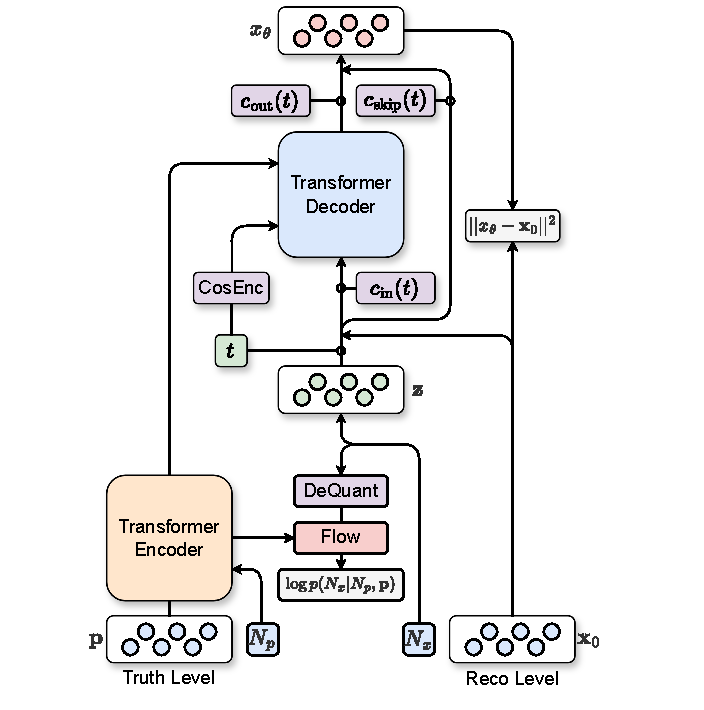
\includegraphics[width=0.70\textwidth]{Figures/jet_generation/PIPPIN.pdf}
    \caption{
        The PIPPIN model architecture which conditionally generates the full set of reconstructed (reco) physics objects from the set of parton-level objects.
    }
    \label{fig:pippin}
\end{figure}

\subsection{Results}

The multiplicity predictor matches the marginals of the true multiplicities to within a few percent, as shown in \Cref{fig:pippin_n}.
Additionally, the predictions are unbiased.
The denoising diffusion model generates reco-level objects with remarkable accuracy to the MC reco-level distributions, as shown in \Cref{fig:pippin_jet}.

In addition to the features of the reconstructed objects, several properties of the underlying decayed particles can be computed.
These include the invariant masses of the W bosons, the top and anti-top quarks, and the full \ttbar system.
To identify the objects originating from each underlying particle, a matching is performed between the partons and the reconstructed objects based on their proximity in $\eta$-$\phi$ space.
These distributions are shown in \Cref{fig:pippin_mass}.

This study compares PIPPIN with two other deep generative models designed for this task, OTUS~\cite{OTUS} and Turbo-Sim~\cite{TurboSim}.
The main metrics are the Kolmogorov-Smirnov distances between the original MC reco-level distributions and the output of the different models.
As shown in \Cref{tab:pippin}, the PIPPIN model outperforms both OTUS and Turbo-Sim in all metrics.

\begin{figure}[htb]
    \centering
    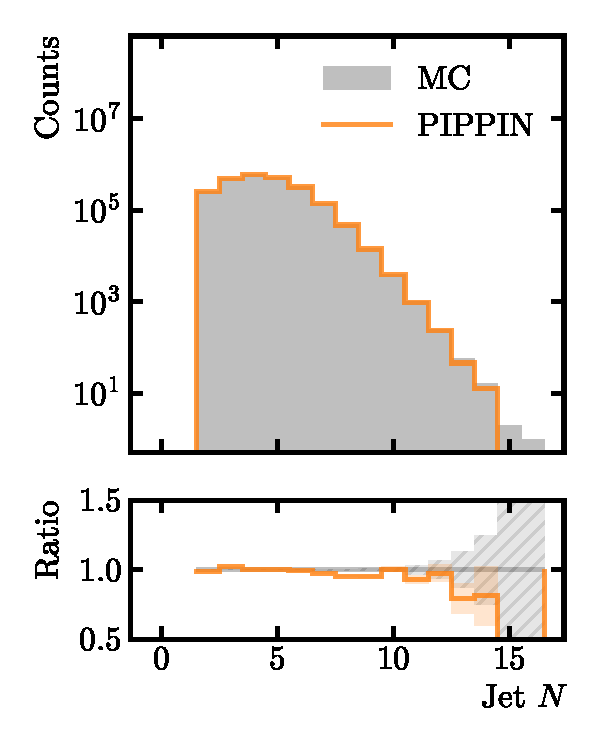
\includegraphics[width=0.32\textwidth]{Figures/jet_generation/pippin/marginals/marginal_jet_n.pdf}
    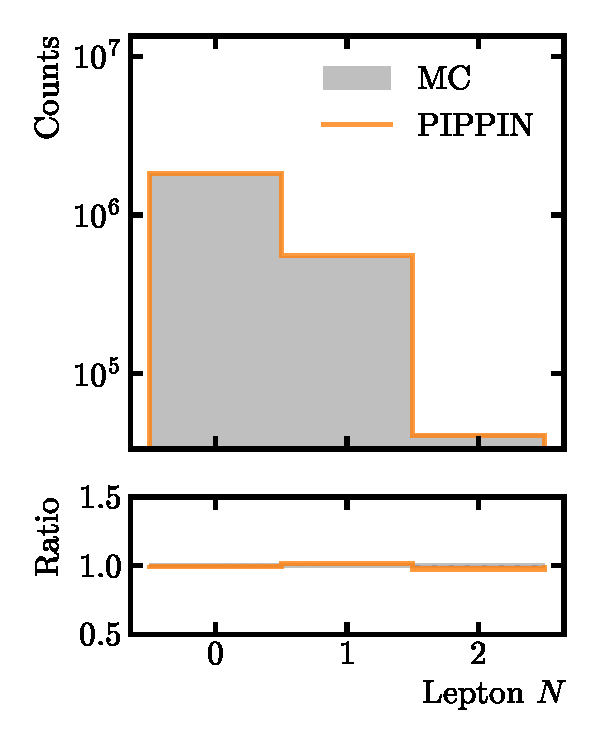
\includegraphics[width=0.32\textwidth]{Figures/jet_generation/pippin/marginals/marginal_lep_n.pdf} \\
    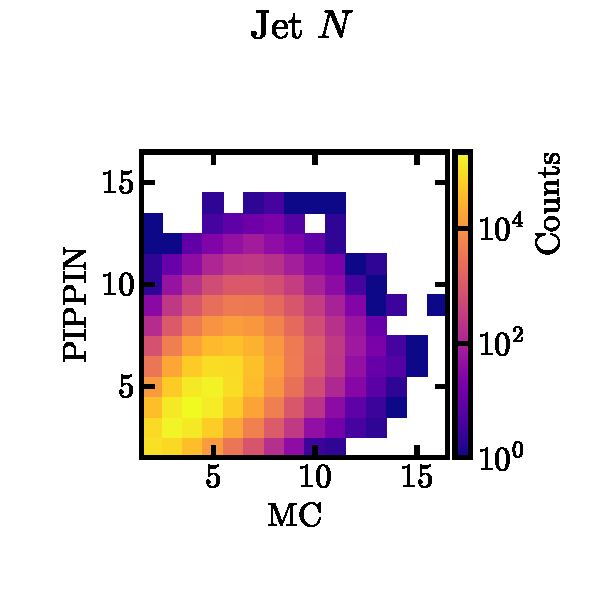
\includegraphics[clip, trim=0cm 0cm 0cm 2.5cm, width=0.32\textwidth]{Figures/jet_generation/pippin/marginals_2D/marginal2D_jet_n.pdf}
    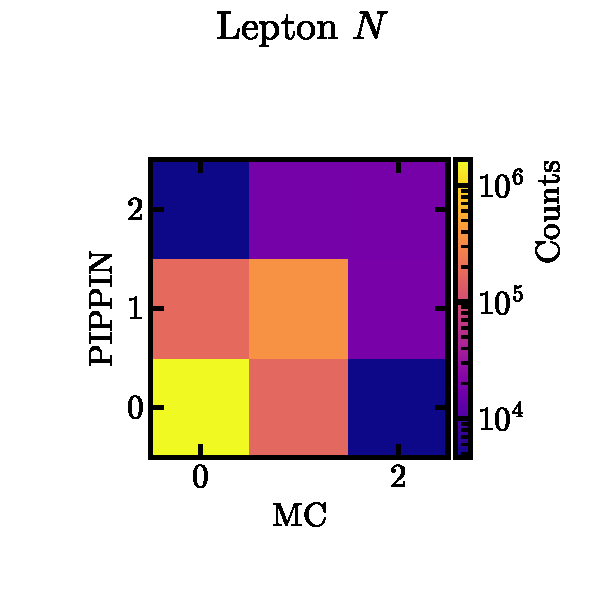
\includegraphics[clip, trim=0cm 0cm 0cm 2.5cm, width=0.32\textwidth]{Figures/jet_generation/pippin/marginals_2D/marginal2D_lep_n.pdf}
    \caption{
        The marginal and conditional distributions of the predicted multiplicities for jets and leptons from the PIPPIN model compared to the full MC pipeline.
    }
    \label{fig:pippin_n}
\end{figure}

\begin{figure}[htb]
    \centering
    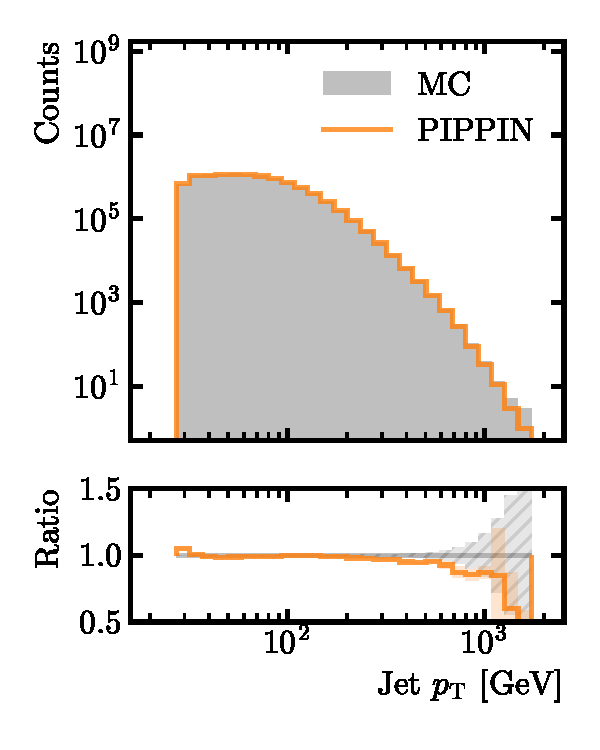
\includegraphics[width=0.32\textwidth]{Figures/jet_generation/pippin/marginals/marginal_jet_pt.pdf}
    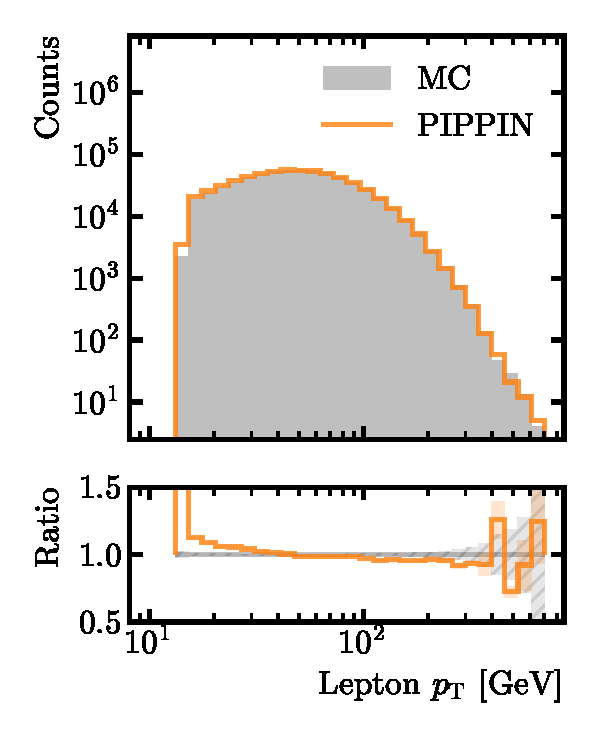
\includegraphics[width=0.32\textwidth]{Figures/jet_generation/pippin/marginals/marginal_lep_pt.pdf}
    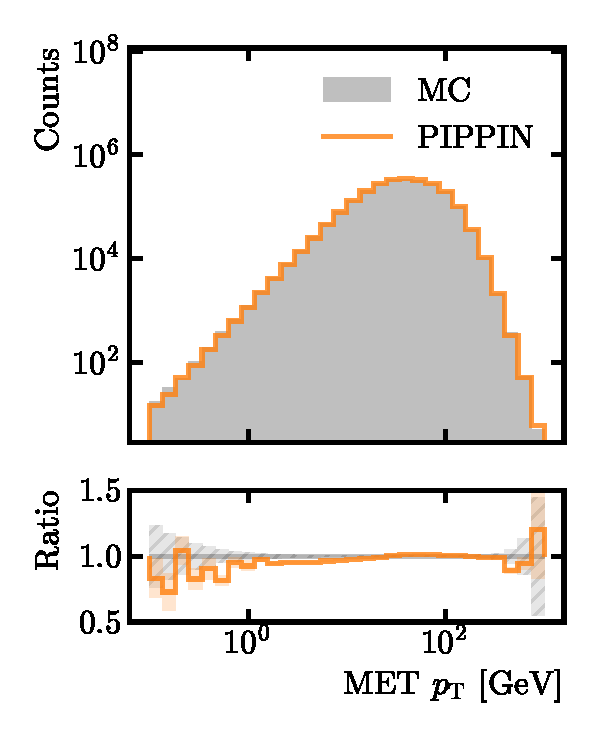
\includegraphics[width=0.32\textwidth]{Figures/jet_generation/pippin/marginals/marginal_met_pt.pdf}
    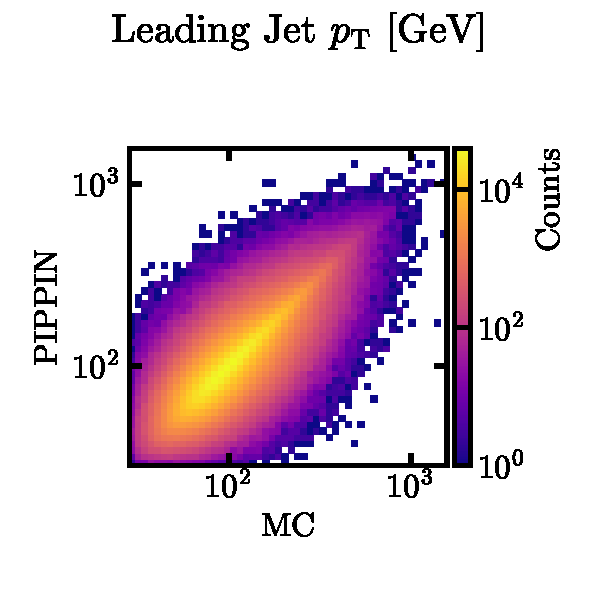
\includegraphics[clip, trim=0cm 0cm 0cm 2.5cm, width=0.32\textwidth]{Figures/jet_generation/pippin/marginals_2D/marginal2D_jet_pt.pdf}
    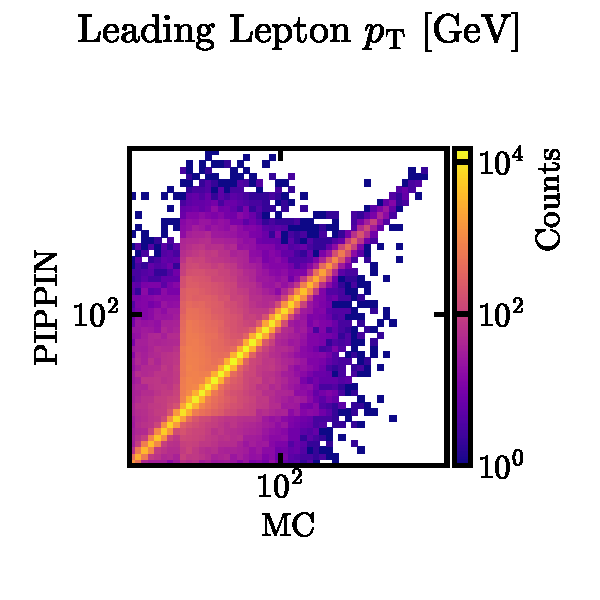
\includegraphics[clip, trim=0cm 0cm 0cm 2.5cm, width=0.32\textwidth]{Figures/jet_generation/pippin/marginals_2D/marginal2D_lep_pt.pdf}
    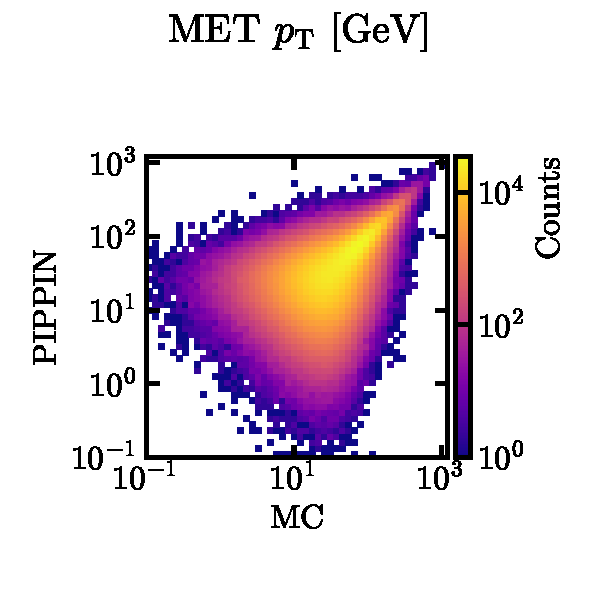
\includegraphics[clip, trim=0cm 0cm 0cm 2.5cm, width=0.32\textwidth]{Figures/jet_generation/pippin/marginals_2D/marginal2D_met_pt.pdf}
    \caption{
        The marginal (top) and conditional distributions (bottom) of the predicted leading jet (left), lepton (middle), and missing \pt (right) from the PIPPIN model compared to the full MC pipeline.
    }
    \label{fig:pippin_jet}
\end{figure}

\begin{figure}[htb]
    \centering
    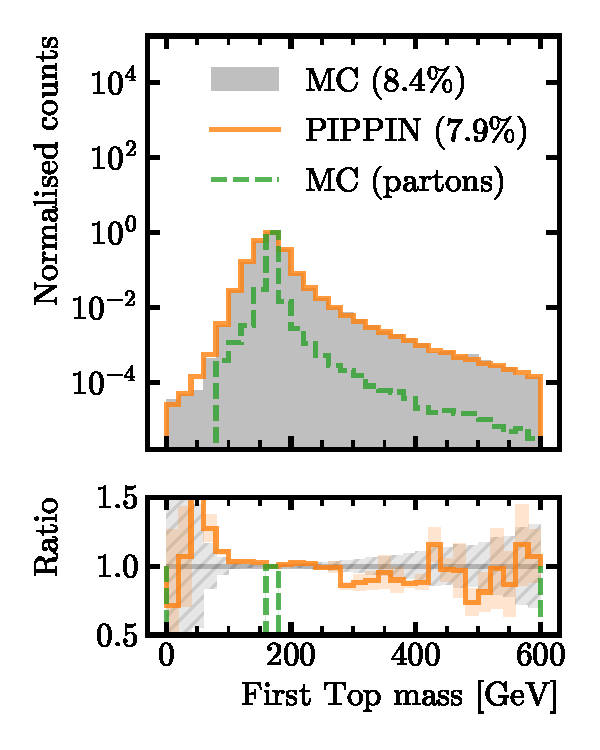
\includegraphics[width=0.32\textwidth]{Figures/jet_generation/pippin/masses/mass_top1.pdf}
    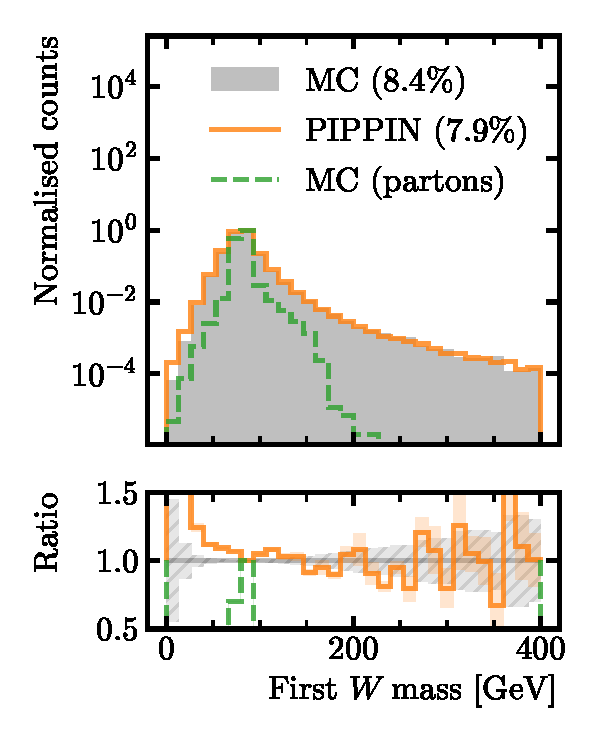
\includegraphics[width=0.32\textwidth]{Figures/jet_generation/pippin/masses/mass_w1.pdf}
    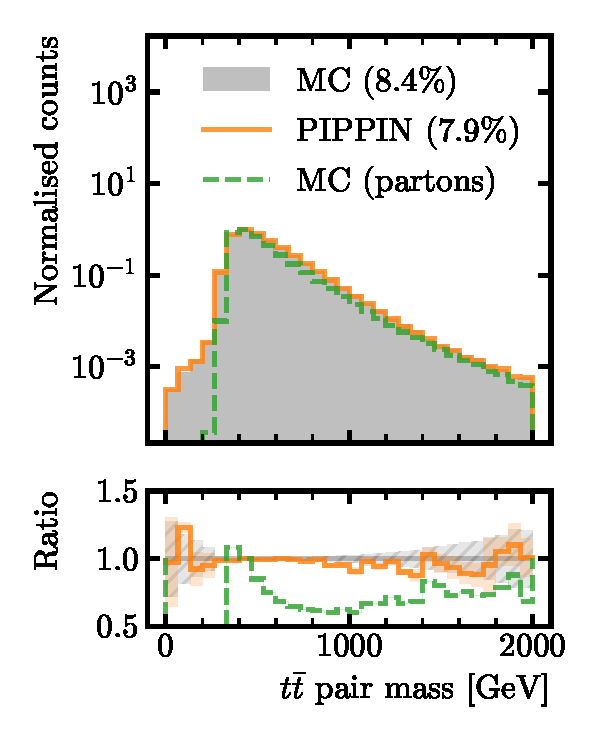
\includegraphics[width=0.32\textwidth]{Figures/jet_generation/pippin/masses/mass_ttbar.pdf}
    \caption{
        The marginal distributions of the reconstructed top quark (left), W boson (middle), and \ttbar (right) invariant masses from the PIPPIN model compared to the full MC pipeline.
        Also shown is the parton-level masses for reference.
        The percentages indicate the proportion of events for which all partons were unambiguously matched and therefore present in these plots.
    }
    \label{fig:pippin_mass}
\end{figure}

\begin{table}[htb]
    \centering
    \renewcommand{\arraystretch}{1.5}
    \caption{Comparison of the PIPPIN model with OTUS and Turbo-Sim on the full forward simulation task. Quoted values are the Kolmogorov-Smirnov distances between the model and the reco-level MC distributions.}
    \label{tab:pippin}
    \begin{tabular}{llllllll}
    \toprule
              & \multicolumn{3}{c}{Reco. objects} & \multicolumn{4}{c}{Underlying particles}                                                                           \\
    \cmidrule(l){2-4} \cmidrule(l){5-8}
    Model     & $p_y^{\text{jet}_1}$              & $p_z^{\text{jet}_1}$                     & $E^{\text{jet}_1}$ & $m^{t\bar{t}}$ & $m^{W_1}$ & $m^{t_1}$ & $m^{t_2}$ \\    \midrule
    OTUS      & 3.78                              & 2.39                                     & 5.75               & 15.8           & 11.7      & 14.1      & 24.9      \\
    Turbo-Sim & 2.89                              & 10.3                                     & 4.43               & 2.97           & 7.72      & 5.20      & 8.52      \\
    PIPPIN    & 0.07                              & 0.14                                     & 0.11               & 0.30           & 1.75      & 0.74      & 0.50      \\
    \bottomrule
\end{tabular}

\end{table}

\FloatBarrier

\subsection{Conclusion}

This study introduces a novel approach to simulating high-energy physics events by utilizing advanced deep learning architectures.
The PIPPIN model directly generates reconstructed objects from final state partons, bypassing the traditional step-by-step pipeline.
The model demonstrates proficiency in addressing the complexity of top quark pair production, accurately predicting both the multiplicity and kinematics of outputs.
It effectively learns the topologies of various decay channels simultaneously, without necessitating channel-specific training.
Additionally, the model captures the correlations between different simulated reconstructed objects, which is crucial for accurate high-energy physics event simulations, as the kinematics of final state particles are interconnected.
One limitation is that only \ttbar events are considered, and it remains to be seen if this can be fully applicable to all physics processes.

The PIPPIN model is also well-suited for the inverse problem of unfolding reconstructed objects to initial partons.
The model could predict the multiplicity of each parton and the correspondence between reconstructed objects and partons, followed by conditional generation with partons as outputs and reconstructed objects as conditional inputs.
The complete application of this method to the unfolding problem remains a subject for future research.

\section{Diffusion for Anomaly Detection}
\label{sec:drapes}

As explained in \Cref{sec:sm_limitations}, there is reason to believe that the current understanding of physics as described by the Standard Model (SM) is incomplete.
However, despite extensive analyses optimized for various beyond the standard model (BSM) signal, no statistically significant evidence of new physics has been found.
Recently, broader anomaly detection methods have gained focus.
These approaches target sensitivity to a much wider spectrum of possible new physics scenarios, at the expense of sensitivity to any one process.

A key technique in many of these model agnostic searches is the \textit{bump hunt}, which searches for localized spikes in data density.
These bumps are often expressed as a resonance in invariant mass, and thus indicative of the decay of a massive particle.
Standard bump hunts are limited by the need to define a signal region (SR) in phase space enriched with enough BSM signal events to be statistically significant over the expected SM background.
Machine learning classifiers can provide a filter to reduce the amount of background present and thus enhance the power of the search.
However, training these models in a signal-agnostic way is challenging.

One such approach is called Classification Without Labels (CWoLa)~\cite{cwola}, whereby a classifier is trained to distinguish between data in the SR against some reference background.
It is assumed that the data in the SR is a mixture of the BSM signal and SM background, denoted as $s+b$.
If the reference background denoted as $b'$ matches exactly the true background $b$, then the optimal classifier that separates $s+b$ from $b'$ is also the optimal classifier for $s$ from $b$.

Constructing the reference background template $b'$ now becomes the central challenge, and several methods have been proposed~\cite{cathode, salad, CURTAINs, feta, lacathode}.
One of the first methods, Cathode~\cite{cathode}, identifies the SR by a slice in some one-dimensional variable $c$, flanked by sidebands (SB).
Each data sample is defined by the slice variable $c$ and additional features $\x$.
A conditional generative model is trained using data from the sidebands to learn $p_\theta(\x|c_{\text{SB}})$, and the template is constructed by sampling from this model using $c$ values in SR, $x_{\text{SR}} \sim p_\theta(\x|c_{\text{SR}})$.
This method is highly effective, provided that the generative model can accurately capture the correlations between $c$ and $\x$, and can interpolate to unseen values of $c_\text{SR}$ during inference.
As long as the signal contamination in the sidebands is much lower than in the SR, the reference background can still lead to a good CWoLa classifier usable for enhanced bump hunts.

This section summarizes the work presented in \textcite{Drapes}, introducing a new model called \drapes.
The \drapes model adapts the approach used in \pcdroid to fill the role of the generative model in the Cathode method using denoising diffusion.

\subsection{Experimental Setup}

This study uses the LHCO R\&D Dataset~\cite{LHCO}, a benchmark for performance in anomaly detection.
The dataset consists of di-jet events, and contains a mixture of a BSM signal and QCD background.
The slice variable $c$ is the di-jet invariant mass, with the SR defined as $m_{jj} \in [3.0, 3.7]~\TeV$.

Two diffusion models are constructed for this task.
One generates only high-level features (\drapes HLV), where $\x$ is a one-dimensional vector, allowing for comparison with previous models which followed the same approach using NFs~\cite{cathode, CURTAINs, lacathode}.
Specifically, these features are:
\begin{equation}
    \x = \left[ m^{1}, \tau_{21}^{1}, \tau_{21}^{2}, \Delta m, \Delta R \right],
\end{equation}
where the superscript denotes the jet number and the $\Delta$ variables measure the difference between the two jets.

The second model, \drapes LLV, generates the di-jet system by individually generating each jet as sets of constituents.
Each jet is defined by up to 150 constituents, similar to JetNet150, resulting in up to 300 individual particles per event.

Both models use the same setup as \pcdroid, but with a basic MLP instead of a transformer encoder for \drapes HLV.
The CWoLa classifier for \drapes HLV is a simple MLP with two hidden layers, while for \drapes LLV, a three-layer transformer with class-attention is used.

Each run of the experiment involved the following steps:
\begin{itemize}
    \item Generate the training set by mixing some signal events with the rest of the QCD background.
    \item Train a background template model using samples from the SB.
    \item Generate the reference background using mass values in the SR.
    \item Train a CWoLA classifier using the reference background and actual data from the SR.
    \item Measure the performance of the classifier at various background rejection rates $r_b$.
\end{itemize}
This entire process is repeated for different levels of signal injection to gauge the model's ability to enhance bump hunts in the presence of different signal strengths.

\subsection{Results}

The primary performance metric, significance improvement ($SIC$), is defined as the number of signal events divided by the square root of the number of background events passing the CWoLA filter.
It is measured for a given background rejection rate ($r_b$).

The high-level template \drapes HLV is compared to the previous state-of-the-art model \FfF.
Both models used the same setup and CWoLA classifier, only the generative model differs.
As upper bounds on performance, two extra classifiers are produced.
The first is a supervised classifier trained using truth labels ($s$ vs $b$).
The second is an idealized CWoLA classifier, trained using true QCD background samples drawn from the SR ($s+b$ vs $b$).
This shows the limits of the CWoLA approach even with perfect background knowledge.
All other classifiers are trained using the reference background $b'$ generated by different methods.

The results on the high-level features are shown in \Cref{fig:drapes_hlv}.
For all levels of initial signal injection, \drapes provides a higher $SIC$ than \FfF.
All template methods, including the idealized classifier, drop off at around 500 injected signal events due to reaching the CWoLA limit of the setup.
This limit is where signal presence is too low compared to the natural fluctuations of the background for a $s+b$ vs $b$ classifier to be able to pick out the signal~\cite{AachenLimit}.

\drapes outperforms the idealized classifier in some cases by increasing the $b'$ statistics through generating more samples, whereas the idealized classifier is limited to the number of QCD events in the dataset.

\begin{figure}[hbpt]
    \centering
    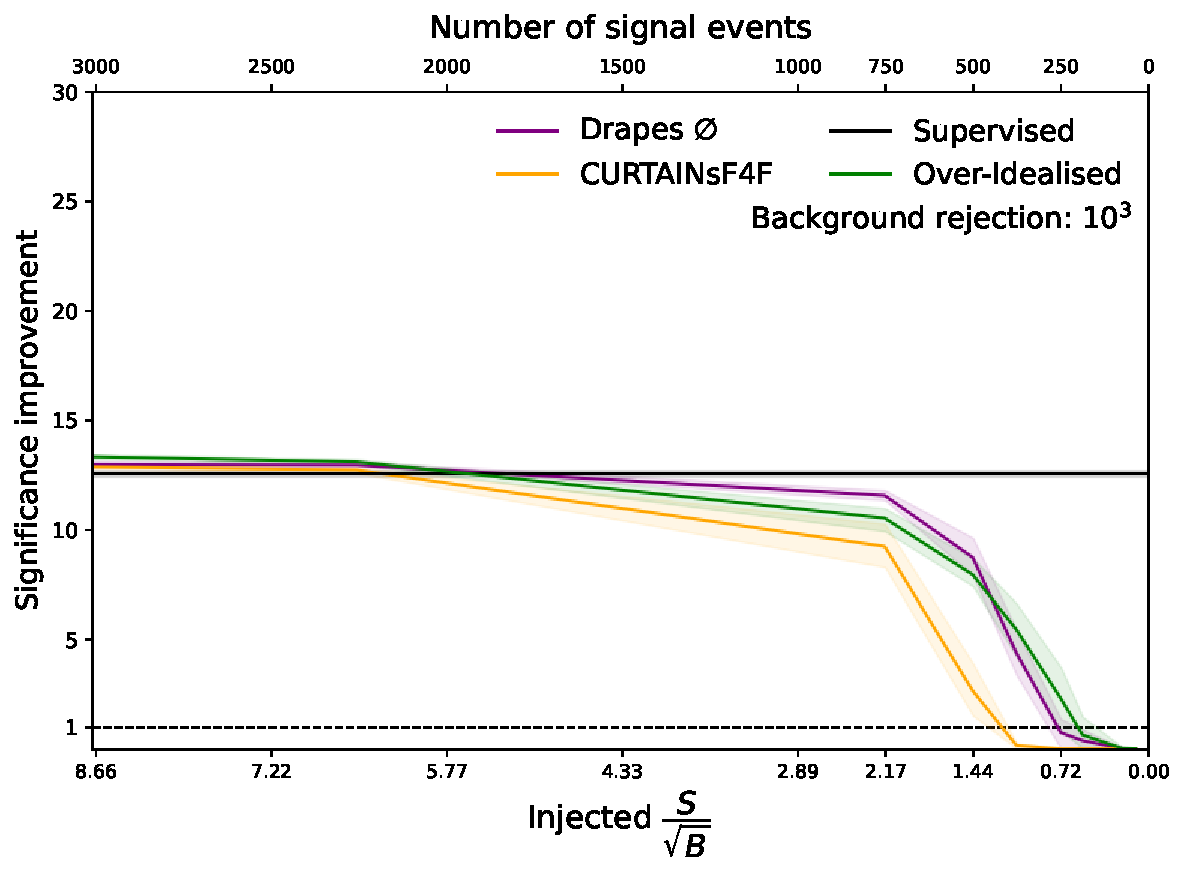
\includegraphics[width=0.49\textwidth]{Figures/jet_generation/drapes/og_compare_rej_1000_sic_vs_nsig.pdf}
    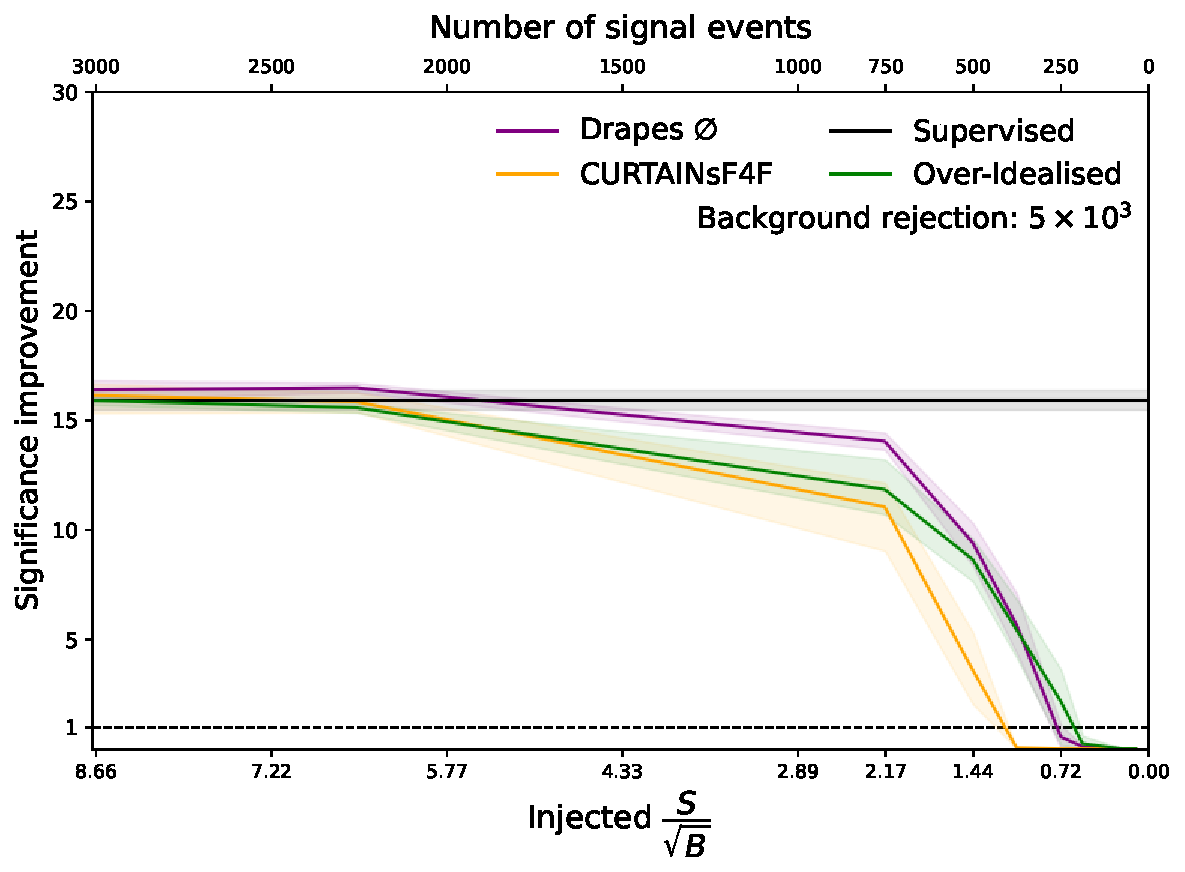
\includegraphics[width=0.49\textwidth]{Figures/jet_generation/drapes/og_compare_rej_5000_sic_vs_nsig.pdf}
    \caption{Significance improvement at fixed background rejection rates of $10^3$ (left) and \mbox{$5 \times 10^3$} (right) as a function of the number of signal events in the signal region, \mbox{$3300\leq m_{jj}<3700~\GeV$}, for \drapes, \FfF, Supervised, and Over-Idealised.
        The injected significance measured from the number of signal and background events in the signal region before applying a cut $\frac{S}{\sqrt{B}}$ is also shown.
        The lines show the mean value of fifty independent classifiers, with the shaded band representing a 68\% uncertainty.
    }
    \label{fig:drapes_hlv}
\end{figure}

The performance of \drapes~(LLV) with varying signal amounts is shown in \cref{fig:drapes_llv}.
When using low-level features, the supervised benchmark yields an $SI=23.5$ at $r_b=1000$, significantly higher than the supervised benchmark using high-level features, which has an $SI=13.5$.
This increase in performance demonstrates the potential sensitivity enhancements for searches operating on low-level features.

\drapes~LLV surpasses the high-level supervised model easily; however, it requires around 2000 signal events injected into the signal region, corresponding to a significance of 5.
At these levels of signal presence, no additional anomaly detection methods would be needed as this excess would easily be detectable in a naive bump hunt.
Unfortunately, the performance of \drapes~LLV drops off significantly below 2000 signal events and becomes worse than the high-level approach in the regions where it is most needed.
This observation aligns with a similar study conducted contemporaneously with this work~\cite{FullPhaseSpace}.

The reason for this drop-off in performance is that CWoLa classifiers using neural networks lose sensitivity as input dimensionality increases, especially with signal-insensitive inputs~\cite{lacathode}.
Moving from a few high-level variables to jet constituents multiplies the input dimensionality by over 150, severely affecting weakly supervised neural networks.
Many new searches revert to decision trees over neural networks for the classifiers as they seem better suited for CWoLa style training~\cite{TreebasedAlgorithmsWeakly, AnomalyDetectionPresence}, but this is not possible for the low-level jet constituents.
More work is therefore needed to find a way to train larger models on point cloud data in a weakly supervised manner.

\begin{figure}[hbpt]
    \centering
    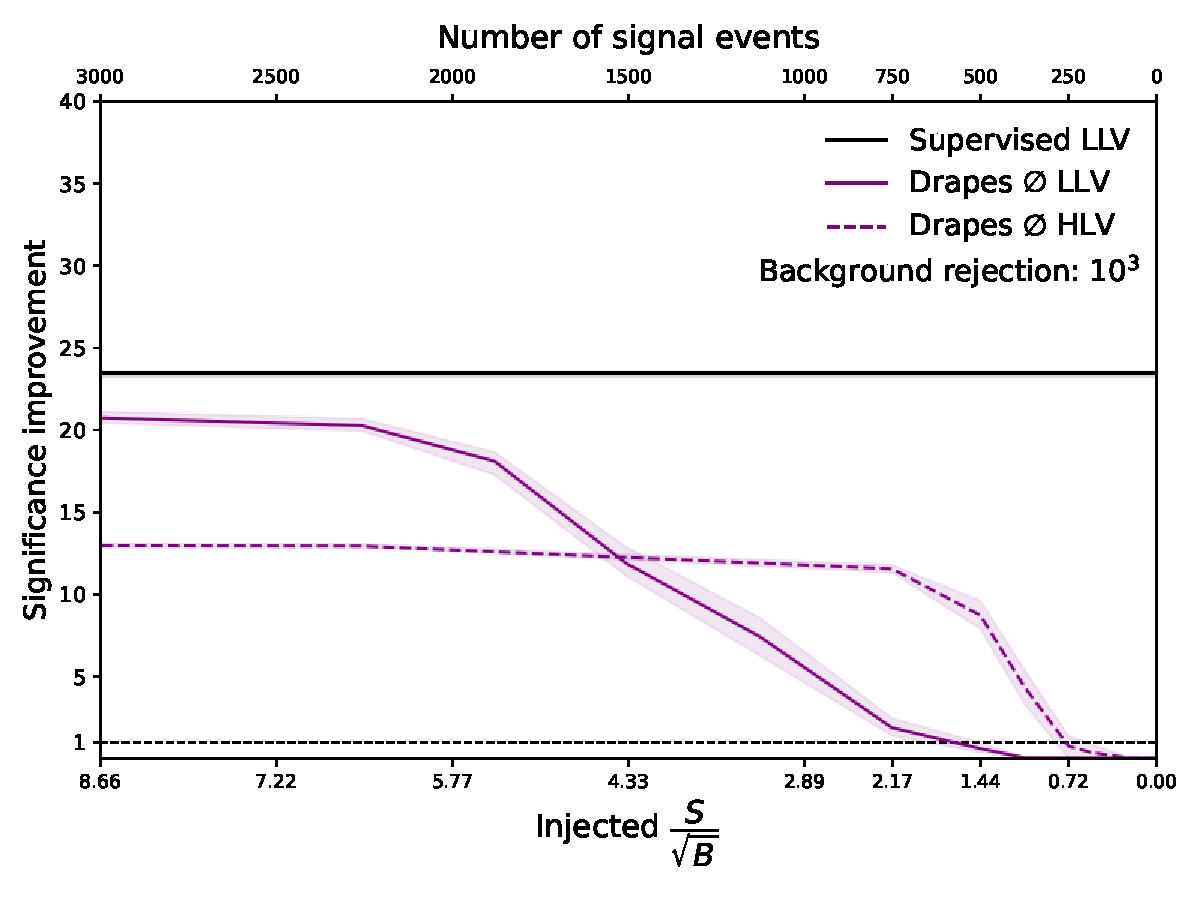
\includegraphics[width=0.49\textwidth]{Figures/jet_generation/drapes/lowlevel_null_sic_vs_soverb_rej_1000.pdf}
    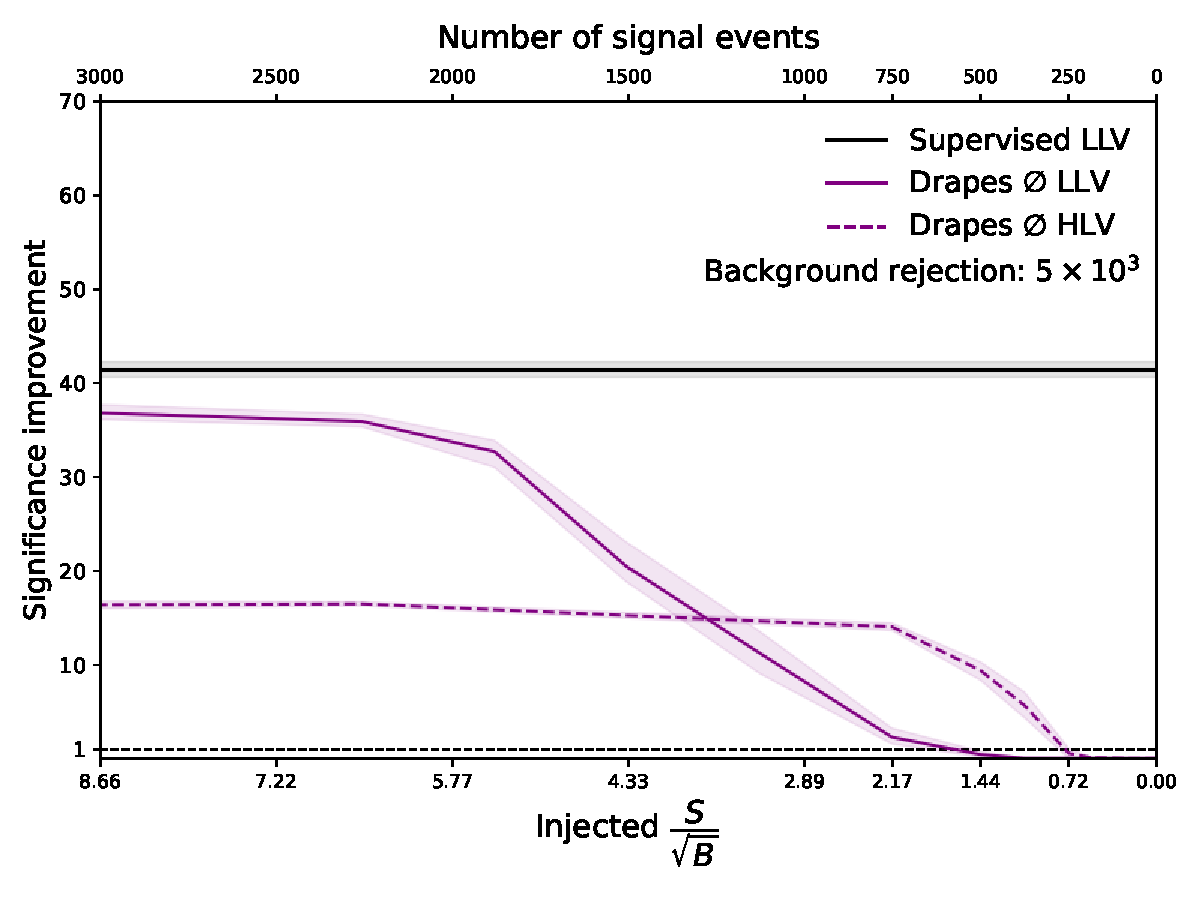
\includegraphics[width=0.49\textwidth]{Figures/jet_generation/drapes/lowlevel_null_sic_vs_soverb_rej_5000.pdf}
    \caption{Significance improvement at fixed background rejection rates of $10^3$ (left) and \mbox{$5 \times 10^3$} (right) as a function of the number of signal events in the signal region, \mbox{$3300\leq m_{jj}<3700~\GeV$}, for \drapes using low level jet constituents (LLV) or high level variables (HLV). The injected significance measured from the number of signal and background events in the signal region before applying a cut $(\frac{S}{\sqrt{B}})$ is also shown. The lines show the mean value of fifty independent classifiers, with the shaded band representing a 68\% uncertainty. The supervised classifier is trained on low level jet constituents is shown for reference.}
    \label{fig:drapes_llv}
\end{figure}

\subsection{Conclusion}

Demonstrating that diffusion models can generate templates for CWoLa classifiers in anomaly detection highlights a significant advancement.
The \drapes HLV generated templates lead to increased sensitivity in CWoLa-style signal searches, surpassing the previous state-of-the-art model \FfF.

However, transitioning to the constituent space reveals a notable drop in sensitivity when the injected signal significance falls below 4.33.
Corroborating studies~\cite{FullPhaseSpace} suggest this decrease is attributable to the challenges faced by a large transformer trained with highly noisy labels, rather than issues with the template generation process.
